\documentclass{article}

% Recommended, but optional, packages for figures and better typesetting:
\usepackage{microtype}
\usepackage{graphicx}
%%\usepackage{subfigure}
\usepackage{booktabs} % for professional tables

\usepackage{stfloats}
% hyperref makes hyperlinks in the resulting PDF.
% If your build breaks (sometimes temporarily if a hyperlink spans a page)
% please comment out the following usepackage line and replace
% \usepackage{icml2025} with \usepackage[nohyperref]{icml2025} above.
\usepackage{hyperref}


% Attempt to make hyperref and algorithmic work together better:
\newcommand{\theHalgorithm}{\arabic{algorithm}}

% Use the following line for the initial blind version submitted for review:
\usepackage[accepted]{icml2025}

% If accepted, instead use the following line for the camera-ready submission:
%\usepackage[accepted]{icml2025}

% For theorems and such
\usepackage{amsmath}
\usepackage{amssymb}
\usepackage{mathtools}
\usepackage{amsthm}

% if you use cleveref..
\usepackage[capitalize,noabbrev]{cleveref}

%%%%%%%%%%%%%%%%%%%%%%%%%%%%%%%%
% THEOREMS
%%%%%%%%%%%%%%%%%%%%%%%%%%%%%%%%
\theoremstyle{plain}
\newtheorem{theorem}{Theorem}[section]
\newtheorem{proposition}[theorem]{Proposition}
\newtheorem{lemma}[theorem]{Lemma}
\newtheorem{corollary}[theorem]{Corollary}
\theoremstyle{definition}
\newtheorem{definition}[theorem]{Definition}
\newtheorem{assumption}[theorem]{Assumption}
\theoremstyle{remark}
\newtheorem{remark}[theorem]{Remark}
\usepackage{bbm}
\newcommand{\x}{\boldsymbol{x}}
\newcommand{\z}{\boldsymbol{z}}
\newcommand{\fix}{\marginpar{FIX}}
\newcommand{\new}{\marginpar{NEW}}
\usepackage{enumitem}
\usepackage{amsthm}
\usepackage{booktabs}
\newcommand{\bftab}{\fontseries{b}\selectfont}
\usepackage{amssymb}
\theoremstyle{plain}
\usepackage{amsmath}
\usepackage{multirow}
\usepackage{tikz}
\usetikzlibrary{automata,arrows,positioning,calc,fit,bayesnet}
\usepackage{graphicx}
\usepackage{subcaption}
\usepackage{booktabs}
\newtheorem{prop}{Proposition}[section]
\renewcommand{\thedefinition}{\arabic{section}.\arabic{subsection}}
\renewcommand{\thetheorem}{\arabic{section}.\arabic{subsection}}
\renewcommand{\thelemma}{\arabic{section}.\arabic{subsection}}
\renewcommand{\theprop}{\arabic{section}.\arabic{subsection}}
\renewcommand{\theremark}{\arabic{section}.\arabic{subsection}}
% Todonotes is useful during development; simply uncomment the next line
\newcommand{\ind}{\perp\!\!\!\!\perp} 
%    and comment out the line below the next line to turn off comments
%\usepackage[disable,textsize=tiny]{todonotes}
\usepackage[textsize=tiny]{todonotes}

\newtheorem{innercustomgeneric}{\customgenericname}
\providecommand{\customgenericname}{}
\newcommand{\newcustomtheorem}[2]{%
  \newenvironment{#1}[1]
  {%
   \renewcommand\customgenericname{#2}%
   \renewcommand\theinnercustomgeneric{##1}%
   \innercustomgeneric
  }
  {\endinnercustomgeneric}
}

\newcustomtheorem{customthm}{Theorem}


\providecommand{\customgenericname}{}
\newcommand{\newcustomlma}[2]{%
  \newenvironment{#1}[1]
  {%
   \renewcommand\customgenericname{#2}%
   \renewcommand\theinnercustomgeneric{##1}%
   \innercustomgeneric
  }
  {\endinnercustomgeneric}
}

\newcustomtheorem{customlma}{Lemma}

% The \icmltitle you define below is probably too long as a header.
% Therefore, a short form for the running title is supplied here:
\icmltitlerunning{Censor Dependent Variational Inference}

\begin{document}

\twocolumn[
\icmltitle{Censor Dependent Variational Inference}

% It is OKAY to include author information, even for blind
% submissions: the style file will automatically remove it for you
% unless you've provided the [accepted] option to the icml2025
% package.

% List of affiliations: The first argument should be a (short)
% identifier you will use later to specify author affiliations
% Academic affiliations should list Department, University, City, Region, Country
% Industry affiliations should list Company, City, Region, Country

% You can specify symbols, otherwise they are numbered in order.
% Ideally, you should not use this facility. Affiliations will be numbered
% in order of appearance and this is the preferred way.
\icmlsetsymbol{equal}{*}

\begin{icmlauthorlist}
\icmlauthor{Chuanhui Liu}{Purdue}
\icmlauthor{Xiao Wang}{Purdue}
\end{icmlauthorlist}

\icmlaffiliation{Purdue}{Department of Statistics, Purdue University, USA}

\icmlcorrespondingauthor{Xiao Wang}{wangxiao@purdue.edu}

% You may provide any keywords that you
% find helpful for describing your paper; these are used to populate
% the "keywords" metadata in the PDF but will not be shown in the document
\icmlkeywords{Machine Learning, ICML}

\vskip 0.3in
]

% this must go after the closing bracket ] following \twocolumn[ ...

% This command actually creates the footnote in the first column
% listing the affiliations and the copyright notice.
% The command takes one argument, which is text to display at the start of the footnote.
% The \icmlEqualContribution command is standard text for equal contribution.
% Remove it (just {}) if you do not need this facility.
\printAffiliations{} 
%\printAffiliationsAndNotice{}  % leave blank if no need to mention equal contribution
%\printAffiliationsAndNotice{\icmlEqualContribution} % otherwise use the standard text.

\begin{abstract}
This paper provides a comprehensive analysis of variational inference in latent variable models for survival analysis, emphasizing the distinctive challenges associated with applying variational methods to survival data. We identify a critical weakness in the existing methodology, demonstrating how a poorly designed variational distribution may hinder the objective of survival analysis tasks—modeling time-to-event distributions. We prove that the optimal variational distribution, which perfectly bounds the log-likelihood, may depend on the censoring mechanism. To address this issue, we propose censor-dependent variational inference (CDVI), tailored for latent variable models in survival analysis. More practically, we introduce CD-CVAE, a V-structure Variational Autoencoder (VAE) designed for the scalable implementation of CDVI. Further discussion extends some existing theories and training techniques to survival analysis. Extensive experiments validate our analysis and demonstrate significant improvements in the estimation of individual survival distributions. Codes can be found at \href{https://github.com/ChuanhuiLiu/CDVI}{https://github.com/ChuanhuiLiu/CDVI}. 
\end{abstract}

\vspace{-5pt}
\section{Introduction}\label{Sec:1}
Survival analysis, a fundamental topic in statistics, finds wide-ranging applications across healthcare, insurance, quality management, and finance. It focuses on modeling the relationship between time-to-event outcomes and individual demographic covariates, where the event of interest could be death, disease progression, or similar occurrences. A key challenge in survival analysis arises from censored observations, which provide only partial information about the survival time, necessitating specialized methods to handle such data effectively.

Deep learning has emerged as a powerful paradigm to advance survival analysis \citep{wiegrebe2024deep}. Recent studies focus on modeling time-to-event distributions via latent variable survival models (LVSMs), applying various probabilistic assumptions and inference techniques. For example, \citet{ranganath2016deep} assumed that the prior of $Z$ belongs to the class of deep exponential family distributions \citep{brown1986fundamentals}. Instead, deep survival machine \citep{nagpal2021dsm} considered the finite discrete latent space, and the time-to-event distribution is one of the finite Gumbel or normal distributions. For discrete time-to-event, \cite{xiu2020variational} modeled a softmax-activated neural network incorporating the Nelson-Aalen estimator \citep{aalen1978nonparametric}, while \citet{Apellániz2024} followed a similar setup, developing variational autoencoders (VAEs) \cite{Kingma2014,rezende2014stochastic} for continuous time-to-event. These new advances of LVSM have demonstrated superior performance across various metrics, including the time-dependent Concordance Index \citep{antolini2005time}, compared to Accelerated Failure Time (AFT) \citep{miller1976least} and Cox Proportional Hazard (CoxPH) \citep{cox1972regression} models. The exacted latent information also enables various downstream tasks based on the extracted latent representation \citep{manduchi2022a}. 

A unique aspect of LVSM optimization is its reliance on variational methods to maintain computational efficiency, due to the intractability of the objective function. Therefore, the variational inference (VI) framework in LVSM is critical to LVSM performance and must be tailored the core task of survival analysis—modeling the time-to-event distribution.


Despite extensive research on the optimality of Variational Inference (VI), its applicability and benefits for time-to-event modeling remain unclear due to the challenges posed by censored data. Furthermore, many aspects of the variational method in existing applications of LVSM remain unclear, including theoretical insights into the inference optimality of LVSM and domain-specific rationales for practical design choices.

This paper provides a comprehensive theoretical analysis of VI optimality and proposes a novel and insightful methodology of LVSM. The paper is organized as follows: Section \ref{sec:2} provides a comprehensive review of LVSM. Section \ref{sec:theory} identifies the limitations of variational methods in existing approaches and introduces censor-dependent variational inference (CDVI). Section \ref{sec:methods} discusses the implementation of CDVI in VAE-based models, offering practical insights and several key implications. Section \ref{sec:exp} validates CDVI and our proposed models through extensive experiments.


\section{Preliminaries}\label{sec:2}

\textbf{Notations}: Random variables (r.v.) are denoted by capital alphabetical letters, e.g. $X,Z,Y,U,C$, and their distribution functions have matching subscripts. $\mathcal{X}$ denotes the sample space of $X$. $P(\cdot), F(\cdot),p(\cdot),S(\cdot),h(\cdot)$ respectively denote a general probability function, a cumulative distribution function, a density function, a survival (tail) function, and a hazard function. Subscripts in Greek letters $\theta,\phi$ denote the unknown parameters. E.g. $S_{Y,\theta}(\cdot)$ refers to the survival function of $Y$ parameterized by $\theta$. Different densities are distinguished by additional letters, such as $f_\theta(\cdot)=p_{U,\theta}(\cdot), q_\phi(\cdot)=p_{Z,\phi}(\cdot)$. A proportional relationship over $x$ is denoted as $\propto_x$.  Estimates of functions or random variables are indicated with a caret or dot symbol above, e.g., $\hat{S}(\cdot)$ is an estimate of $S(\cdot)$. $\log$ denotes natural logarithms. Bold symbol $\x$ denotes vectors. 





\subsection{Right-censoring and Partial Log-likelihood}\label{sec:2.1}

In survival analysis tasks, we are given a dataset consisting of $n$ triplets $\{\x_i,y_i,\delta_i\}_{i=1}^n$. In a single-event right-censoring setting, the event indicator $\delta_i$ is binary valued. In particular, $\delta_i=1$ signifies that $y_i$ is the observed time of the event of interest (time-to-event), while $\delta_i=0$ signifies that $y_i$ is right-censored and the true time-to-event of subject $i$ exceeds the observed value. 

We assume the dataset consists of i.i.d. random variables $\{X,Y,I\}$, where $Y$ is the continuous observed survival time, $I$ is the binary event status, and $X$ represents individual feature. Notably, $(Y,I)$ is considered as surjective maps of two continuous random variables $(U,C)$, where $U$ is the \underline{u}ncensored time-to-event and $C$ is the \underline{c}ensoring time. Specifically, assume that $U\ind C|X$, we define
\begin{equation}
    Y= \min(U,C),~~ \ I=\mathbbm{1}(U \leq C).
\end{equation}
For any data triplet $\{\x,y,\delta\}$, the parameters $\theta,\eta$ for $U,C$ determine the \textit{density}\footnote{Radon–Nikodym derivative of the distribution $P(Y,I|X)$ w.r.t. the product of the Lebesgue and counting measure.} of $y,\delta$ conditioned on $\x$. The logarithm of the partial likelihood $p_{U,\theta}(y|\x)^{\delta}S_{U,\theta}(y|\x)^{1-\delta}$, while not a proper density, defines the objective function $L(\theta)$ for time-to-event modeling. Formally, it is given as
\begin{equation}\label{parametricloss}
\begin{aligned}
        L(\theta)&: ={\delta}\log f_{\theta}(y|\x) + (1-\delta)\log S_{\theta}(y|\x),
\end{aligned}
\end{equation}
where $f_{\theta}(y|\x)=p_{U,\theta}(y|\x)$ and $S_{\theta}(y|\x)$ represent the density and survival functions of $U$ evaluated at $y$, respectively.

\subsection{Latent Variable Survival Model}
LVSMs construct $f_{\theta}(u|x)$ from \eqref{parametricloss} within a latent structure using a continuous latent variable $Z$, enabling a more flexible and expressive characterization than traditional methods. As shown in Fig.\ref{fig:graph}, it is given by
\begin{equation}\label{survivaldensity}
    f_{\theta}(u|\x) 
=\int_{z\in \mathcal{Z}} f_{\theta}(u|\x,\z) \pi_{\theta}(\z|\x) dz.
\end{equation}
We refer to $\pi_{\theta}(\z|\x)$ as the prior of $Z$.
Especially, an AFT model can be interpreted as LVSM in a d-separation latent structure, as illustrated in Fig \ref{fig:graph}.b, constrained by a linear latent, e.g., $Z|X=\alpha+\beta^\top X$. 
\begin{figure}[!ht]
\subfloat[generative graph of LVSM]{
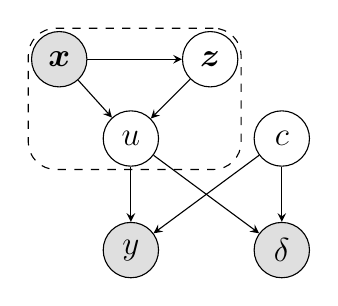
\begin{tikzpicture}[> = stealth,  auto,   node distance = 2.5cm,box/.style = {draw,dashed,inner sep=1pt,rounded corners=10pt}]
        \node[latent] (z) {\large $\z$};
        \node[obs] (x) [left =1.2cm of z] {\large $\x$};
        \node[latent] (u) [below left=0.5cm and 0.5cm of z] {\large $u$};
        \node[latent] (c) [right = 1.2cm of u] {\large $c$};
        \node[obs] (y) [below =0.7cm of u] {\large $y$};
        \node[obs] (i) [below =0.7cm of c] {\large $\delta$};
        \node[box,fit=(x)(u)(z)] {};
		\path[->] (x)  edge node{} (u);
            \path[->] (x)  edge node{} (z);
		\path[->] (z) edge node{} (u);
            \path[->] (u)  edge node{} (y);
            \path[->] (u)  edge node{} (i);
            \path[->] (c) edge node{} (y);
            \path[->] (c) edge node{} (i);
\end{tikzpicture}}
\hspace*{\fill}
  \subfloat[latent structure of $Z$]{
      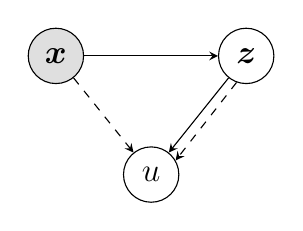
\begin{tikzpicture}[> = stealth,  auto,   node distance = 2.5cm,box/.style = {draw,dashed,inner sep=2pt,rounded corners=15pt}]
        \node[latent] (z) {\large $\z$};
        \node[obs] (x) [left =1.7cm of z] {\large $\x$};
        \node[latent] (u) [below left=1cm and 0.7cm of z] {\large $u$};
            \path[->] (x)  edge node{} (z);
		\path[->] (z) edge node{} (u);
            \path[->,dashed] (x)  edge node{} (u);
		\path[->,dashed] (z.250) edge node{} (u.30);
      \end{tikzpicture}}
\hspace*{\fill}
\caption{Directed acyclic graphs of LVSM. The shaded nodes $\x,y,\delta$ are observed. (a) The dashed box shows a general generative graph of $U$. (b) D-separation, denoted in solid line, assumes $X \perp U\mid Z$; Dashed line shows a V-structure graph, assuming a $X$-independent latent $Z$.}
\label{fig:graph}
\vspace{-5pt}
\end{figure}


While LVSM is more flexible, the M-estimation of $\theta$, i.e., $\hat{\theta}_{mle}=\arg\max L(\theta)$ is challenging due to its computational cost. Specifically, $f_\theta$ in \eqref{parametricloss} may lack a closed-form integral, rendering it even harder to approximate $S_\theta$ reliably.

\vspace{-5pt}
\subsection{Vanilla Variational Inference for LVSM}\label{sec.VanillaVI}
As a solution, VI is one of the common techniques in LVSM. Here, we review a general framework of VI, referred to as the \textbf{Vanilla VI}, as seen in \citet{ranganath2016deep, xiu2020variational, Apellániz2024}. Specifically, unbiased tractable estimators are proposed via a variational distribution $q_\phi(\z|\x,y)$. By Jensen's inequality, $\log f_\theta(y|x)$, $\log S_\theta(y|x)$ in Eq.~\ref{parametricloss} can be lower bounded by 
\begin{equation}\label{lowerbound}
\hspace{-7pt} \log f_\theta(y|x)\geq \mathbb{E}_{q_\phi}\log f_\theta(y|\x,\z) - \text{KL}[q_\phi||\pi_\theta(\z|\x)], 
\end{equation}
\begin{equation}\label{lowerbound2}
\hspace{-5pt} \log S_\theta(y|\x)\geq \mathbb{E}_{q_\phi}\log S_\theta(y|\x,\z) - \text{KL}[q_\phi||\pi_\theta(\z|\x)].
\end{equation}
The expectation of the plug-in estimator $\hat{L}(\theta)$ yields the lower bound of $L(\theta)$, which is given by in \citet{xiu2020variational},
\begin{equation}\label{originalelbo}\begin{aligned}
    &\text{ELBO}(\theta,\phi) := \delta \mathbb{E}_{q_\phi}\log f_\theta(y|\x,\z) \\&+ (1-\delta)\mathbb{E}_{q_\phi}\log S_\theta(y|\x,\z)-\text{KL}[q_\phi||p_\theta(\z|\x)].
\end{aligned}
\end{equation}
In case that $p_\theta(\z | \x)$ is intractable, \citet{ranganath2016deep,Apellániz2024} further decomposed the $\text{KL}[q_\phi||p_\theta(\z|\x)]$ (KLD) as shown below. The intractable $\log p_\theta(\x)$ is moved into $L(\theta)$ by rearrangement.
\begin{equation}\label{lowerbound3}
    \text{KLD} =\log p_\theta(\x)+\text{KL}[q_\phi||\pi(\z)]-\mathbb{E}_{q_\phi}\log p_\theta(\x|\z).
\end{equation} 
When the distributions in \eqref{originalelbo} (and \eqref{lowerbound3}) are tractable, efficient computation of both the expectation and KL divergence improves scalability for large datasets. Often, optimizing $\text{ELBO}(\theta,\phi)$ can be done by amortized black-box VI algorithms \citep{ranganath2014black} via the reparameterization trick \citep{Kingma2014,rezende2014stochastic}.

\vspace{-5pt}
\subsection{Variational Inference Optimality}\label{VanillaVI}
The key distinction in ELBO optimization lies in its pursuit of two distinct objectives \textit{simultaneously}: 1) the M-estimation of $\theta$ and 2) the variational bound of the partial log-likelihood. The second objective aims to minimize the \textit{inference gap} \citep{cremer2018inference}, i.e., bias, of $L(\theta)$: 
\begin{equation}\label{infgap}
    B(\theta,\phi) := L(\theta)-\text{ELBO}(\theta,\phi).
\end{equation}
Since the optimum $(\theta^*,\phi^*):=\arg\max \text{ELBO}(\theta,\phi)$ balances the best of these two results, the accuracy of $\theta^*$ inherently relies on the optimality of VI. 
A suboptimal VI solution leads to a significant and irreducible inference gap, i.e., $\min_{\phi}B(\theta,\phi)\gg 0$, which prevents $\theta^*$ from correctly recovering true M-estimator $\hat{\theta}_{mle}$. Consequently, improper variational approximations introduce bias and degrade the reliability of parameter estimates.

Obviously, common knowledge of VI in a supervised setting, such as optimal $q_\phi(\z|\x,y)$ being related to intractable posterior $p_\theta(\z|\x,y)$, fails to extend to survival analysis. That said, variational methods proposed in existing applications lack adequate depth and often are counter-intuitive from a Bayesian perspective, leaving ambiguity about their purpose and effectiveness. For example, \citet{nagpal2021dsm} adopted a lazy strategy in obtaining $q_\phi$, where $q_\phi$ is manually set to be the tractable $p_\theta(z|x)$. Similarly, \citet{Apellániz2024} limited $q_\phi$ to depend on $X$ only, making it completely ignore the information of $y$. 

\vspace{-5pt}
\section{Theories}\label{sec:theory}
This section focuses on the foundational theories of the inference optimality for LVSM in a single-event right-censoring scenario, assuming at least one censored and one uncensored survival time are observed. The results are formulated without taking into account the practical limitations.
\subsection{Problems in vanilla VI}\label{sec:3.1}
We start by analyzing the equality conditions of Eq.~\ref{lowerbound} and Eq.~\ref{lowerbound2} \textit{without} censoring involved. The notation $u$ here stresses the dependency on $U$ instead of survival time $Y$.
\begin{lemma}[\textbf{Equality conditions of Eq.~\ref{lowerbound} and Eq.~\ref{lowerbound2}}]\label{lemma1}
\ \\
Given any parameter $\theta$, the point-wise equality in Eq.~\ref{lowerbound} holds for any $\{X=\x,U=u\}$, if and only if one of the following conditions holds: 
\begin{enumerate}[nosep,label={(\alph*)}]
\setlength\itemsep{0em}
\item $q_\phi(\z|\x,u)=f_{\theta}(u,\z|\x)/f_\theta(u|\x)$, where  $f_\theta(u,\z|\x)$ $:= f_\theta(u|\x,\z)\pi_\theta(\x|\z)$; \label{itm:1}
\item $\exists$ \text{map} $c_1$,  $f_{\theta}(u,\z|\x)/q_\phi(\z|\x,u) = c_1(\x,u)$; \label{itm:2}
\item $ \mathrm{KL}[q_\phi(\z|\x,u)||p_{\theta}(\z|\x,u)] = 0$. \label{itm:3}
\end{enumerate}% 
Likewise, Eq.~\ref{lowerbound2} holds for any $\{X=\x,U=u\}$, if and only if the following equivalent conditions hold:
\begin{enumerate}[nosep,label={(\alph*')}]
\item  $q_\phi(\z|\x,u)=S_{\theta}(u,\z|\x)/S_\theta(u|\x)$, where we abuse $S_\theta(u,\z|\x):=\int_{s=u}^\infty f_\theta(s,\z|\x)ds$; \label{itm:4}
\item $\exists$ \text{map} $c_2$, $S_{\theta}(u,\z|\x) /q_\phi(\z|\x,u) = c_2(\x,u)$. \label{itm:5}
\end{enumerate}%
\end{lemma}

The conditions for Eq.~\ref{lowerbound} follow the standard VI argument, and the conditions for Eq.~\ref{lowerbound2} are derived under the additional assumption of Fubini's Theorem.  
As these two conditions differ, a natural question arises: \textit{Given any $\theta$ and $(\x,u)$, what kind of $q_\phi(\z|\x,u)$ would satisfy both conditions?}  

Perhaps surprisingly, Proposition \ref{thm1} below shows that these conditions are more than conflicting, leading to notorious issues. For notation clarity, let $\Phi_1(\theta)$ denote the set of $\phi$ where Eq.~\ref{lowerbound} holds equal, $\Phi_2(\theta)$ denote the one for Eq.~\ref{lowerbound2}, so $\Phi_{U}(\theta):=\Phi_1(\theta)\cap \Phi_2(\theta)$ is the ideal parameter set for optimal $q_\phi$ with no constraints. We define $\Theta_U := \{\theta\mid \Phi_{U}(\theta) \neq \varnothing \}$ to denote the support set of $\theta$. 

\begin{prop}[\textbf{Degradation for optimal $q_\phi(z|x,u)$}] \label{thm1}\ \\
Assuming that 1) optimal VI is feasible: $\Theta_U  \neq \varnothing$, and 2) $f_\theta(u|\x,\z)$ is a location-scale density with location $\mu_\theta(\x,\z)$ and scale $\sigma$. Then, given any $x,u$,
\begin{enumerate}[nosep,label={(\arabic*)}]
\item \textbf{Latent non-identifiability:} $\forall \theta \in \Theta, h_{\theta}(u|\z,\x)$ is indepedent of $\z$;\label{itm:6}
\item \textbf{Location degradation:} $\forall \theta \in \Theta$, location parameter $\mu_{\theta}(\x,\z)$ is independent of $\z$; \label{itm:7}
\item \textbf{Lazy posterior:} $\forall \theta \in \Theta$, $\forall \phi \in \Phi_{U}(\theta)$, the variational distribution $\textup{KL}[q_{\phi}(\z|\x,u)\lVert \pi_{\theta}(\z|\x)] = 0$; \label{itm:8}
\item \textbf{Surely posterior collapse:} If $ \z \perp\!\!\!\!\perp \x$, $\forall \theta \in \Theta, \phi \in \Phi_{U}(\theta)$, $\textup{KL}[q_{\phi}(\z|\x,u)\lVert \pi(\z)] = 0$. \label{itm:9}
\end{enumerate}%
\end{prop}
To be specific, claims \ref{itm:6} and \ref{itm:7} assert that $h_\theta(u|\x,\z)$, or equivalently $f_\theta(u|\x,\z)$, is independent of $\z$, disregarding the latent information from prior $\pi_\theta(\z|\x)$. Remarkably, such behavior of $f_\theta(u|\x,\z)$, called \textit{latent non-identifiability} \citep{wang2021latent}, is first identified in survival analysis. Furthermore, under the location-scale, i.e., distribution assumption of $f_\theta(u|\x,\z)$, its mean $\mu_\theta(\x,\z)$ reduces to a univariate function, restricting LVSM to a non-linear AFT regression. This observation may have explained why most of the applications assume a d-separation latent structure, where $f_\theta(u|\x,\z)$ is fully dependent on $z$, to mitigate or avoid issues in claim \ref{itm:7}. As we mentioned in Section \ref{sec.VanillaVI}, the fact that optimal VI can only be achieved on extremely limited support of $\theta$ is devastating: optimizing ELBO may inadvertently shift towards its secondary objective.


Moreover, claim \ref{itm:8} demonstrates the negligibility of the optimal $q_\phi$, i.e., such $q_{\phi}$ collapses to the conditional prior $\pi_\theta(\z|\x)$, ignoring the information of $u$. The reason is simple---since both $f_{\theta}(u|\x,\z)$ and $S_{\theta}(u|\x,\z)$ are independent of $\z$, their posterior equals nothing but their common prior. To this extent, the optimal $q_{\phi}$ becomes as lazy as the one in \citet{nagpal2021dsm}. It also explains the rationale in \citet{Apellániz2024}, where the proposed $q(\z|\x)$ is not dependent on $u$. Such an effect can be more detrimental in a V-structure, e.g., the latent $\z$ represents an unseen individual-independent treatment. Claim \ref{itm:9} states that optimal $q_\phi$ is the prior $\pi(\z)$, which leads to a notorious issue called posterior collapse.

We are now ready to incorporate the censored data. Indeed, Eq.~\ref{lowerbound} and Eq.~\ref{lowerbound2} have different supports, namely, the event space $\mathcal{D}_E$ and the censored space $\mathcal{D}_C$, 
\begin{equation}
\begin{aligned}
\mathcal{D}_E&:=\{(x,y) \mid (x,y,1)\in \mathcal{X}\times \mathcal{Y}\times \mathcal{I} \},\\
\mathcal{D}_C&:=\{(x,y) \mid (x,y,0)\in \mathcal{X}\times \mathcal{Y}\times \mathcal{I} \}.  
\end{aligned}
\end{equation}
\begin{remark}\label{rmk4.1} 
For any ${(x,y)}\in \mathcal{D}_E\cap \mathcal{D}_C$, Proposition \ref{thm1} is applicable to the optimal $q_\phi$. 
\end{remark}

Remark \ref{rmk4.1} delineates the conditions under which Proposition \ref{thm1} extends to censored data. Specifically, given the data triplets $\{\x,y,0\}$ and $\{\x,y,1\}$, the optimal variational distribution $q_\phi$ that simultaneously satisfies both cases encounters challenges within the framework of Proposition \ref{thm1}.
Thus, if they are disjoint, e.g., by a Type-I censoring, it is \textit{theoretically} possible for vanilla VI to achieve a zero inference gap, satisfying the conditions of Eq.~\ref{lowerbound} on $\mathcal{D}_E$ and Eq.~\ref{lowerbound2} on $\mathcal{D}_C$. That said, the type of censoring and its effect on the partition of the sample space are crucial to the vanilla VI optimality. 

It should be stressed that the non-informative censoring assumption, containing random censoring, independent censoring, and Type-I censoring, is too general to define in its influence on the partition of the sample space and vanilla VI optimality. While it is commonly used in the existing literature, the optimality of vanilla VI can vary significantly across these cases. Evident in benchmark datasets (See Table \ref{tab:dataset_rw}), observational studies rarely have disjoint spaces; vanilla VI is at least suboptimal in these benchmark datasets.

\subsection{Censor-dependent Variation Inference}\label{4.2}

We now establish a less restrictive VI framework for LVSM. 

\begin{customthm}{3.2.1}[\textbf{Point-wise optimal VI}]\label{Thm1}\ \\ 
Given $x,y,\delta$ and parameter $\theta$, the variational distribution $q_\phi(z|x,y,\delta)$ is optimal if and only if for almost every $z\in \mathcal{Z}$, $$q_{\phi^*}(z|x,y,\delta)= \lim_{\Delta z \to 0}P_{\theta,\eta}(z\leq Z\leq z+\Delta z|x,y,\delta)/\Delta z .$$ 
Moreover, if $\mathcal{D}_E= \mathcal{D}_C = \mathcal{X}\times \mathcal{U}$, the optimal $q_{\phi^*}$ is independent of parameters of the censoring distribution $\eta$ , and for almost every $z\in \mathcal{Z}$,

\begin{enumerate}[nosep,label={(\alph*)}]
\setlength\itemsep{0em}
\item $ q_{\phi^*}(z|x,y,1)=q_{\phi^*_1}(z|x,u)|_{u=y}$, where $\phi_1^*\in\Phi_1(\theta)$. 
\item $q_{\phi^*}(z|x,y,0)=q_{\phi^*_2}(z|x,u)|_{u=y}$, where $\phi_2^*\in\Phi_2(\theta)$. 
\end{enumerate}% 
\end{customthm}

Thm \ref{Thm1} states that the optimal density $q_\phi$ is equal to the posterior density of $P(Z|X,Y,\delta)$. In particular, if there is no overlap of sample spaces due to censoring, the optimal $q_\phi$ is the one satisfying Lemma \ref{lemma1}. 

\begin{remark}[\textbf{Vanilla VI propose a marginal $q_\phi$}]\label{rmk4.2}\ \\
Assuming that there is no partition $\mathcal{D}_E= \mathcal{D}_C = \mathcal{X}\times \mathcal{U}$, the marginalized $q_{\phi^*}(z|x,y)$ equals $q_{\phi^*_i}(z|X=x,U=y)$ for any $i=1,2$ if and only if $P(\delta=2-i|Y=y)=1$.
\end{remark}
Remark \ref{rmk4.2} offers an alternative perspective on Remark \ref{rmk4.1}, i.e., the design of $q_\phi$ in Vanilla VI is at fault. To be specific, the inability of vanilla VI to obtain equality in both \eqref{lowerbound} and \eqref{lowerbound2} arises from defining $q_\phi$ as a \textit{marginal} distribution while expecting it to behave as a conditional one. To this extent, further limitations on $q_\phi$ described in Section \ref{sec.VanillaVI}, such as employing a lazy strategy, are irrational.

Remark \ref{rmk4.2} also implies, when there is no disjoint sample subspace, vanilla VI is as optimal as CDVI if and only if there is an absence of event or censoring data. 
\begin{definition} \label{def:cdvi} 
The censor-dependent variational distribution $q_{\phi_1,\phi_2}$ is 
\begin{equation}\label{splitencoder}
    q_{\phi_1,\phi_2}(z|x,y,\delta) := q_{\phi_1}(z|x,y)^{\delta} q_{\phi_2}(z|x,y)^{1-\delta}.
\end{equation}
\end{definition}
Then, the likelihood estimators derived from $q_{\phi_1,\phi_2}$ are
\begin{equation}\label{likelihoodestimator}
\begin{aligned}
\hat{f}_1(z) &:= f_\theta(y,z|x)/q_{\phi_1}(z|x,y), \\
\hat{S}_1(z) &:= S_\theta(y,z|x)/q_{\phi_2}(z|x,y).    
\end{aligned}
\end{equation}
Compared to Vanilla VI, we name it \textit{censor-dependent} because of the necessary dependency of $q_{\phi_1,\phi_2}(z|x,y,\delta)$ on the indicator $\delta$. We use $\phi_1$ and $\phi_2$ for notation purposes, and the subscript $1$ for further discussions. Of importance, it leads to \textbf{Censor-dependent ELBO}:
\begin{equation}\label{elboloss}
\begin{aligned}
  &\text{ELBO-C}:=\delta [\mathbb{E}_{q_{\phi_1}}\log f_{\theta}(y|x,z) -\text{KL}[{q_{\phi_1}}\Vert \pi_\theta(z|x)]]\\&\  +
      (1-\delta) [\mathbb{E}_{q_{\phi_2}}[\log S_{\theta}(y|x,z)]- \text{KL}[{q_{\phi_2}}\Vert  \pi_\theta(z|x)]].
 \end{aligned}  
\end{equation}
Next, we show its suitability for optimal VI and how it resolves the previous issues. For brevity, an informal theorem is presented below, with the formal version in Appendix~\ref{Ap.A2}. Let $\Phi_{P}(\theta)= \{(\phi_1,\phi_2)\mid \phi_1\in \Phi_1( \theta),\phi_2\in \Phi_2( \theta)\}$ denote the set of optimal parameters of CDVI.
\begin{customthm}{3.2.2}[\textbf{Informal; CDVI optimality}] \label{thm3.2.2}\ \\
If $\Phi_{P}(\theta) \neq \varnothing$, $\forall (\phi_1,\phi_2)\in \Phi_{P}(\theta)$, $q_{\phi_1,\phi_2}(z|x,y,0)\propto_z h_{\theta}(y|x,z)q_{\phi_1,\phi_2}(z|x,y,1)$ and $q_{\phi_1,\phi_2}$ do not have issues in proposition \ref{thm1} on a larger support of $\theta$.\end{customthm}

In a nutshell, Thm \ref{thm3.2.2} highlights that CDVI formulates ELBO-C through a properly designed $q_{\phi_1,\phi_2}$, which eliminates the problematic constraint $\theta_1=\theta_2$.

To conclude, our analysis has shown that the vanilla VI framework described in \citet{ranganath2016deep,xiu2020variational,nagpal2021dsm,Apellániz2024} is insufficient and arguably inappropriate for LVSM. Without hindering the M-estimation of $\theta$ and the expressiveness of latent survival models, we have shown the importance of the censoring mechanism and CDVI for optimal VI in LVSM. 
\section{Methods}\label{sec:methods}
In this section, we propose a novel implementation of CDVI in VAE-based LVSMs, as well as share insights into ELBO optimization and CDVI augmentation techniques.
\subsection{Censor-dependent Conditional VAE}\label{sec:cdcvae}
\begin{figure}[!ht]
\subfloat[Vanilla CVAE]{
      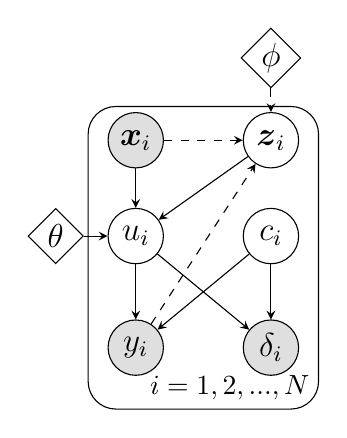
\begin{tikzpicture}[> = stealth,  auto,   node distance = 2.5cm,box/.style = {draw,inner sep=7pt, xshift=0pt, yshift= -5pt, rounded corners=10pt}]
        \node[latent] (z) {\large $\z_i$};
        \node[obs] (x) [left =1.0cm of z] {\large $\x_i$};
        \node[latent] (u) [below =0.5cm of x] {\large $u_i$};
        \node[latent] (c) [right = 1.0cm of u] {\large $c_i$};
        \node[det] (theta) [left = 0.3cm of u] {\large $\theta$};
        \node[det] (phi) [above = 0.3cm of z] {\large $\phi$};
        \node[obs] (y) [below =0.7cm of u] {\large $y_i$};
        \node[obs] (i) [below =0.7cm of c] {\large $\delta_i$};
        \node[box,fit=(x)(y)(c)] (fit){};
        \node[above left] at (fit.south east) {$i=1,2,...,N$};
		\path[->] (x)  edge (u);
		\path[->] (z) edge  (u);
            \path[->] (theta)  edge  (u);
            \path[->] (u)  edge node{} (y);
            \path[->] (u)  edge node{} (i);
            \path[->] (c) edge node{} (y);
            \path[->] (c) edge node{} (i);
            \path[->,dashed] (x) edge (z);
            \path[->,dashed] (y) edge (z);
            \path[->,dashed] (phi) edge (z);
      \end{tikzpicture}}
\subfloat[Censor-dependent CVAE]{
      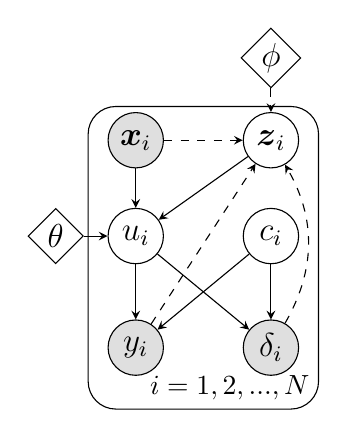
\begin{tikzpicture}[> = stealth,  auto,   node distance = 2.5cm,box/.style = {draw,inner sep=7pt, xshift=0pt, yshift= -5pt, rounded corners=10pt}]
        \node[latent] (z) {\large $\z_i$};
        \node[obs] (x) [left =1.0cm of z] {\large $\x_i$};
        \node[latent] (u) [below =0.5cm of x] {\large $u_i$};
        \node[latent] (c) [right = 1.0cm of u] {\large $c_i$};
        \node[det] (theta) [left = 0.3cm of u] {\large $\theta$};
        \node[det] (phi) [above = 0.3cm of z] {\large $\phi$};
        \node[obs] (y) [below =0.7cm of u] {\large $y_i$};
        \node[obs] (i) [below =0.7cm of c] {\large $\delta_i$};
        \node[box,fit=(x)(y)(c)] (fit){};
        \node[above left] at (fit.south east) {$i=1,2,...,N$};
		\path[->] (x)  edge (u);
		\path[->] (z) edge  (u);
            \path[->] (theta)  edge  (u);
            \path[->] (u)  edge node{} (y);
            \path[->] (u)  edge node{} (i);
            \path[->] (c) edge node{} (y);
            \path[->] (c) edge node{} (i);
            \path[->,dashed] (x) edge (z);
            \path[->,dashed] (i) edge [bend right=30] (z);
            \path[->,dashed] (y) edge (z);
            \path[->,dashed] (phi) edge (z);
      \end{tikzpicture}}
\hspace*{\fill}
\caption{Implementations of Vanilla VI and CDVI.}
\label{fig:cvae}
\end{figure}


We propose the Censor-dependent Conditional VAE (CD-CVAE) that estimates parameters $\theta,\phi$ as weights of neural networks. As shown in Fig.\ref{fig:cvae}, our proposed CDVI implementation incorporates both $y$ and the event indicator $\delta$ as input of the encoder. Fig.\ref{fig:cdcvae} illustrates that its decoder leverages a V-structure and employs both Gaussian and Gumbel-minimum distribution families of $\varepsilon$, interpretable as an infinite LogNormal or Weibull mixture survival regression on positive survival time.
\begin{figure}[!ht]
\hspace*{\fill}
\subfloat[The encoder]{
      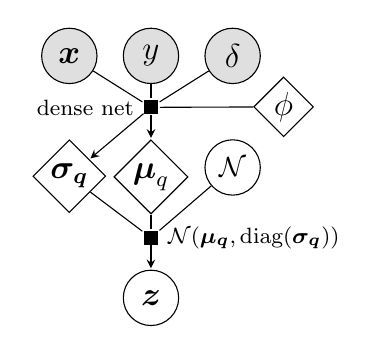
\begin{tikzpicture}[> = stealth,  shorten > = 0.5pt,   auto,   node distance = 2.5cm,box/.style = {draw,inner sep=6pt,xshift=5pt,rounded corners=10pt}]
        \node[obs] (y) {\large $y$};
        \node[obs] (i)[right =0.32cm of y] {\large $\delta$};
        \node[obs] (x)[left =0.32cm of y] {\large $\x$};
        \node[det] (phi)[below right =0.2cm and 0.2cm of i] {\large $\phi$};
        \node[det] (sigma)[below =0.7cm of x] {\large $\boldsymbol{\sigma_q}$};
        \node[det] (mu)[below =0.7cm of y] {\large $\boldsymbol{\mu}_q$};
        \node[latent] (normal)[below =0.7cm of i] { $\mathcal{N}$};
        \node[latent] (z) [below =0.7cm of mu]{\large $\z$};
        \factor[below=0.2cm of y] {sigma-factor} {left: dense net} {} {}
        \factoredge {x,y,i,phi} {sigma-factor} {sigma,mu};
        \factor[below=0.2cm of mu] {z-factor} {right:$\mathcal{N}(\boldsymbol{\mu_q},\textup{diag}(\boldsymbol{\sigma_q})$)} {} {}
        \factoredge {mu,sigma,normal} {z-factor} {z} ; %        
      \end{tikzpicture}}
\subfloat[The decoder]{
      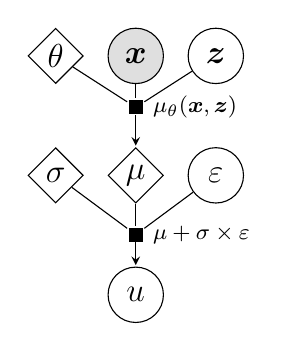
\begin{tikzpicture}[> = stealth,  shorten > = 0.5pt,   auto,   node distance = 2.5cm,box/.style = {draw,inner sep=6pt,xshift=5pt,rounded corners=10pt}]
        \node[obs] (x) {\large $\x$};
        \node[latent] (z)[right =0.3cm of x] {\large $\z$};
        \node[det] (theta) [left=0.3cm of x] {\large $\theta$};
        \node[det] (mu) [below =0.8cm of x] {\large $\mu$};
        \node[det] (sigma) [left=0.3cm of mu] {\large $\sigma$};
        \node[latent] (eps) [right=0.3cm of mu] {\large $\varepsilon$};
        \node[latent] (u) [below=0.8cm of mu]{\large $u$};
        \factor[below=0.3cm of mu] {u-factor} {right:$\mu+\sigma\times\varepsilon$} {} {}
        \factoredge {mu,sigma,eps} {u-factor} {u} ; %
        \factor[below =0.2cm of x] {mu-factor} {right:$\mu_\theta(\x,\z)$} {} {}
        \factoredge {x,z,theta} {mu-factor} {mu} ; %
      \end{tikzpicture}}
\hspace*{\fill}
\caption{Generative graph of CD-CVAE.}
\label{fig:cdcvae}
\vspace{-5pt}
\end{figure}

\subsection{Training Strategy of Decoder Variance}
As shown in Fig.\ref{fig:cdcvae}b, $\sigma$ is an \textit{independent} model parameter that is \textit{jointly} updated with all other parameters. Here, we emphasize in Prop.\ref{prop:mle} that the estimate of decoder variance \textit{cannot} be obtained in closed form. Consequently, a dual-step algorithm that updates it separately, as seen in \citet{rybkin2021simple} and \citet{liu2025doubly}, is not applicable to VAE-based LVSM, although it is preferred. For notation clarity, we decompose $\theta=\{\zeta,\sigma\}$ in this subsection. 



\begin{prop}[\textbf{No closed form update of $\sigma$}]\label{prop:mle}
Given the dataset $\{\x_i,y_i,\delta_i\}$ and $\zeta,\phi_1,\phi_2$, the optimum of $\sigma$ by $\frac{\partial \textup{ELBO-C}(\theta,\zeta,\sigma)}{\partial\sigma} = 0$ has no closed-form solution. In particular, if $\varepsilon$ follows a normal distribution, we have
$$
\frac{\partial\textup{ELBO-C}}{\partial\sigma}=\mathbb{E}_q[\sum_{i: \delta_i=1}\frac{\tilde{y}^2_i}{\sigma}-\frac{1}{\sigma})+\sum_{i:\delta_i=0} h(\tilde{y}_i)\frac{\tilde{y}_i}{\sigma}],
$$
where $\tilde{y}=(y-\mu_\zeta(\x,\z))/\sigma$ is the location-scale standardized time $y$.
\end{prop}

\subsection{Augmented CDVI and the implementations}
This section formulates different log-likelihood estimators, and its expectation as ELBO and introduces the variant of our proposed model, adopting established VI techniques: 1) importance sampling and 2) delta methods to generalize CDVI, 


\begin{definition}[Importance weighted estimator for CDVI] \label{def5.2}
Following Definition \ref{def:cdvi}, the unbiased Monte Carlo estimators of likelihood $f_\theta(y|x), S_\theta(y|x)$ are defined as 
\begin{equation}\label{importantsampled}
\hat{f}_m:=\frac{1}{m}\sum_{i=1}^m \hat{f}_1(\z_i),~\hat{S}_k:=\frac{1}{k}\sum_{j=1}^k\hat{S}_1(\z_j),
\end{equation} 
where $\z_i$ and $\z_j$ are independent samples from $ q_{\phi_1,\phi_2}$, assuming $\delta =1,0$, respectively. 
\end{definition}
As expected, \eqref{importantsampled} defines a general $\hat{L}_{m,k} := \log(\hat{f}_m ^\delta\hat{S}_k^{1-\delta})$ for $L(\theta)$. Computing its expectation allows us to generalize \eqref{elboloss} to $\text{ELBO-C}_{(m,k)}$, as well as \eqref{infgap} to $B(m,k)$

Next, we establish 3 key results about the properties of $\hat{L}_{m,k}$, providing deeper insights into augmented CDVI in both the finite $m,k$ case and the asymptotic regime as $m,k \to \infty$.

\begin{customthm}{4.3.1}[\textbf{Monotonicity of $B(m,k)$}] \label{thm4.3.1}\ \\
Given any $\theta,\phi$, for any $m\in \mathbb{N}_+, k\in \mathbb{N}_+$,\\
$
\begin{aligned}
B(1,1)&\geq  B(m,k):=L(\theta) - \textup{ELBO-C}_{m,k}(\theta,\phi)\\
&\geq \max(B(m,k+1),B(m+1,k))\\ &\geq B(m+1,k+1) \geq \lim_{m',k'\to \infty}B(m',k') = 0  
\end{aligned}$
\end{customthm}

The dependency of $B(m,k)$ on model parameters $\theta,\phi$ is omitted; $B(1,1)$ is equal to the gap of \eqref{elboloss} in Thm \ref{thm4.3.1}.

Thm \ref{thm4.3.1} generalizes the well-known property of \citet{burda2015importance} to CDVI. Specifically, we prove that the generalized inference gap $B(m,k)$ is monotonic in both size $m$ and $k$. In other words, $\text{ELBO-C}_{m,k}$ yields a smaller inference gap for any $m>1,k>1$ given a \textit{fixed} $\theta,\phi_1,\phi_2$, which vanishes as $m,k \to \infty$. That said, Thm \ref{thm4.3.1} holds for any $\phi_1,\phi_2$, including the constrained ones  ${\phi_1}=\phi_2$, as seen in \citet{xiu2020variational}. 

\begin{customthm}{4.3.2}
[\textbf{Self-normalized Importance Sampling}] \label{thm4.3.2}
Let $Q_{1}(m),Q_{2}(k)$ be the augmented variational distribution, and $P_{1}(m),P_{2}(k)$ be the augmented posterior distribution, defined as follows:
\begin{equation}
\begin{aligned}
&J_{1}(m)=\hat{f}_1\textstyle \prod_{i=1}^m q_{\phi_1}(z_i|x,y),\ Q_{1}(m)= J_{1}(m)/\hat{f}_m \\
&J_{2}(k)= \hat{S}_1\textstyle \prod_{j=1}^k q_{\phi_2}(z_j|x,y),\ Q_{2}(k)= J_{2}(k)/\hat{S}_k\\
&P_{1}(m)\propto_{z_{1:m}} J_{1}(m),\ P_{2}(k)\ \propto_{z_{1:k}} J_{2}(m).\\
\end{aligned}
\end{equation}
Then, given any $x,y,\delta$, 
\begin{equation}
\begin{aligned}
 &L(\theta)-\mathbb{E}_{Q_1,Q_2}[\hat{L}_{m,k}]\\&= \textup{KL}[Q_{1}(m)||P_{1}(m)]^\delta  \textup{KL}[Q_{2}(k)||P_{2}(k)]^{(1-\delta)}.
\end{aligned}
\end{equation}
\end{customthm}
Thm \ref{thm4.3.2} extended and corrected the results from \citet{Domke2018}, formulating augmented CDVI as another lower bound and KL divergence. This result generalizes the established connection of self-normalized importance sampling (SNIS) to CDVI. For example, $(\hat{f}_1/\hat{f}_m)$ can be seen as a self-normalized weight.  However, as we point out, it does not enable a direct comparison between $B(m,k)$ and $B(1,1)$, since the expectation is taken over $Q_1$ and $Q_2$. Detailed discussion can be found in Appendix \ref{AP.B6}. 

\begin{customthm}{4.3.3}[\textbf{Informal; Consistency}] \label{thm4.3.3}\ \\
Under some moment assumptions, for $m\to\infty,k\to \infty$, the variance of $\hat{L}_{m,k}$ goes to zero, and thus $\hat{L}_{m,k}$ is a biased yet consistent estimator of $L(\theta)$, i.e., for any $\xi>0$,
$$\lim_{m,k\to\infty}P(|\hat{L}_{m,k}-L(\theta)|>\xi)=0.$$
\end{customthm} 
Despite that Thm \ref{thm4.3.1} has shown a vanishing bias of $\hat{L}_{m,k}$, Thm \ref{thm4.3.3} quantifies the asymptotic behavior of its variance, thereby establishing its consistency. This result is extended from \citet{nowozin2018debiasing}, enhancing CDVI under ideal assumptions with theoretical guarantees. Thm \ref{thm4.3.3} also leads to the tradeoff of unbiasedness and asymptotic bias below.
\begin{definition}[Delta method estimator for CDVI] \label{ue} \ \\
A biased variant of Definition \ref{def5.2} is defined as
\begin{equation}\label{dviestimator}
\quad \dot{f}_m:=\exp\{\hat{\alpha}_2/(2m\hat{f}^2_m)\}\hat{f}_m, \\
\end{equation}
\begin{equation}\label{dviestimator2}
\dot{S}_k:= \exp\{\hat{\beta_2}/(2k\hat{S}^2_k)\}\hat{S}_k,
\end{equation} where we define $\hat{\alpha}_2$ and $\hat{\beta}_2$ as the corresponding sample variances of $\{\hat{f}_1(\z_i)\}_{i=1}^m$ and $\{\hat{S}_1(\z_i)\}_{i=1}^k$, e.g., $\hat{\alpha}_2:=\frac{1}{m-1}\textstyle \sum_{i=1}^m(\hat{f}_1(\z_i)-\hat{f}_m)^2$.
\end{definition}

We show in Appendix~\ref{Ap.a4} that the Delta method \cite{teh2006collapsed} induced log-likelihood estimator $\dot{L}_{m,k}$ enjoys less asymptotic bias of $L(\theta)$ compared to \eqref{importantsampled}, if $m,k$ are sufficiently large. 

\section{Experiments}\label{sec:exp}
We refer to the above-mentioned techniques as $\text{IS}$, and $\text{DVI}$. 
The additional details of experiments are in Appendix~\ref{Ap.C}. 
\subsection{Evaluation Metrics}

\textbf{Concordance index} \cite{harrell1982evaluating} :
Concordance measures the effectiveness of a discriminative model in ranking survival times correctly. Specifically, it assesses whether the model assigns a shorter predicted time to the event, $\hat{u}_i$, or a lower survival probability, $\hat{S}(t|x_i)$, at any test time $t$, for a subject with features $x_i$ who experienced the event at time $u_i$, compared to a subject with features $x_j$ who survived longer.
Due to censoring, only comparable pairs $y_i \leq y_j,\delta_i =1$ are considered. Thus, Harrell's $C$-index is defined as:
\begin{equation*}
    C(t)=P(\hat{S}(t|x_i)\leq\hat{S}(t|x_j) \mid y_i \leq y_j,\delta_i =1).
\end{equation*}
We evaluate the trained models by calculating the average C-index over ten quantiles, ranging from $10^{th}$ to $100^{th}$ quantile in increments of 10, of event test times.

\textbf{Brier score} \cite{graf1999assessment}:  It is a weighted squared prediction error reweighted by Inverse Probability of Censoring Weighting (IPCW), which assesses the model's conformity/calibration, as well as prediction accuracy. 
\begin{equation*}
\begin{aligned}
\textup{Brs}(t)&= \frac{1}{n} \sum_{i=1}^{n} []
\mathbbm{1}(y_i \leq t ,\delta_i = 1) \frac{(0 - \hat{S}(t | \x_i))^2}{\hat{S}_C(y_i)}\\
&\quad + \mathbbm{1}(y_i > t) \frac{(1 - \hat{S}(t | \x_i))^2}{\hat{S}_C(t)}],    
\end{aligned}
\end{equation*}
where $\hat{S}_C(\cdot)$ is the estimated survival distribution of the censoring random variable $C$. We evaluate the Brier score at the 75th quantile of event time on the test dataset.

\textbf{Time-dependent C-index} \cite{antolini2005time}: Compared to the Harrell's $C$-index, it considers a more limited yet practical set of comparable pairs, where selected subjects who developed the event earlier can't survive longer than the event horizon $t$. Formally, it is defined as  
\begin{equation*}
    C^{td}(t)=P(\hat{S}(t|x_i) \leq \hat{S}(t|x_j)| y_i \leq y_j,\delta_i =1, y_i \leq t).
\end{equation*}
Following conventions, we set the event horizon at the 75th quantile of the event time, and we compute it using IPCW and truncations, aiming to obtain an unbiased estimate of $u_i<u_j$ by giving more weight to test samples with similar features that are not censored. 

\subsection{Inference Optimality on Simulated Datasets}
\begin{table}[!ht]
    \centering
    \caption{Summary table for simulated datasets (SD1-SD6). Sample size for each dataset is $10,000$. Event/Censored time refers to sample statistics of $Y$. The generated samples of $U$ is independently sampled across each datasets. The starting point of Gibbs sampling is fixed at $\z=(0,0)$.}\label{tab:simulate_ds}
    \resizebox{\columnwidth}{!}{
    \begin{tabular}{r|rrrrrr}
        \bftab{Summary} & \bftab{SD1} & \bftab{SD2} & \bftab{SD3} & \bftab{SD4} & \bftab{SD5} & \bftab{SD6}\\ \hline\\[-2.3ex]
        Censor rate    & 0\%    & 5\%    & 20\%  & 30\%  & 50\%  &  100\% \\
        Population mean $\mu_C$& --     & 16.00   & 8.50  &5.50    &0.00     &16.00 \\ 
        Censored time mean  & --     & 2.99   & -0.11  & -1.51  & -4.49   & 16.18 \\ 
        Event time median     & 1.43   & 1.29   & 0.41   &-0.30   & -3.13   & --  \\ 
        Event time min        & -12.64 & -15.85 & -22.47 & -22.59 & -24.28  & -- \\ 
        Event time max        & 21.27  & 21.60  & 17.49  & 18.45  & 14.29   & -- \\ 
    \end{tabular}}
\end{table}
Firstly, we investigate whether amortized CDVI can practically reduce the inference gaps compared to the vanilla VI. Table \ref{tab:simulate_ds} provides a detailed view of population parameters and sample statistics of 6 simulated datasets. To be specific, we use Gibbs sampling, where the true posterior is known and predefined. Both $P(Z|X,Y,I=1)$ and $P(Z|X,Y,I=0)$ are set to normal distributions, which enable the closed-form computation of the inference gaps. We vary the mean of censoring time $\mu_C$ to generate datasets with different censoring rates, in which $C$ follow an independent normal distribution. The values of the censoring rate are rounded, with an error of 1\%.

\begin{table}[!ht]
    \centering
    \caption{Variational inference on simulated datasets. E-KL/C-KL: the average KL divergence between the encoder and true posterior of all Events/Censoring observations in the dataset. Lower is better. We set $m=k=10$.}\label{tab:simulate_vi}
    \resizebox{\columnwidth}{!}{
    \begin{tabular}{r|rr|rr|rr|rr}
          \multirow{2}{*}{\bftab{Data}} &  \multicolumn{2}{c|}{\bftab{CD-CVAE}} &   \multicolumn{2}{c|}{\bftab{CVAE}} & \multicolumn{2}{c|}{\bftab{CD-CVAE}$^{\scalebox{.5}{+\text{IS}}}$}  & \multicolumn{2}{c}{\bftab{CD-CVAE}$^{\scalebox{.5}{+\text{IS}+\text{DVI}}}$}\\ 
        \                 & E-KL   & C-KL    &  E-KL   & C-KL  & E-KL   & C-KL & E-KL   & C-KL \\    \hline    \\[-2.3ex]
        \bftab{SD1}      & 1.65 & --   & 1.65 &  --   & \bftab 1.53 & -- &  1.56 & --  \\
        \bftab{SD2}      & \bftab 1.66 & \bftab 1.93 & 1.75 &  2.70 &  1.64 & 2.17& 1.66 & 2.55 \\ 
        \bftab{SD3}      & 2.38 & 3.13 & 2.79 & 3.18  & 2.23  & 3.21 & \bftab 2.17  & \bftab 3.13\\ 
        \bftab{SD4}      & 2.88 & 3.89 & 3.45 & 4.04  & 2.64  & 4.09 & \bftab 2.29  & \bftab 3.60 \\ 
        \bftab{SD5}      & 4.45 & 5.55 & 5.42 & 5.86  & 4.11  & 5.56 & \bftab 3.89 & \bftab 5.51\\ 
        \bftab{SD6}      & --   & .0871& --  & .0871 & --   & .0862 & --   &  \bftab.0848 \\ 
    \end{tabular}}
    \vspace{-5pt}
\end{table}

Our proposed baseline model CD-CVAE, as shown in Table \ref{tab:simulate_vi}, significantly reduces the average KL divergence between the learned posterior and the true posterior in both event and censoring subsets, and so the inference gap, which is a weighted sum of these two metrics. Leveraging VI improvement techniques, CD-CVAE further reduces the inference gap across various settings of censoring. 

In cases of extreme censoring/event scenarios, where $Y$ is manually set to $U$ or $C$, CD-CVAE performs identically to CVAE, which is expected by Remark \ref{rmk4.2}. Interestingly, all models perform considerably better in the all-event scenario compared to the all-censoring scenario, and neither IS nor DVI yields significant performance improvements. Although learning a data-independent distribution of $C$ should be simpler, such a large discrepancy between these two extreme cases may imply that the amortization effect \cite{cremer2018inference} can dominate the inference gap. This observation highlights potential opportunities for practical inference improvements of amortized CDVI. 

During the experiment, we also found that CD-CVAE models can converge to various local optima with nearly the same inference gap, while having different ratios of E-KL and C-KL. This observation implies a unique trade-off in the amortization CDVI, i.e., the censor/event KL trade-off. A follow-up work on the interpretation of such trade-off would be meaningful.

\begin{table}[!ht]
    \centering
    \caption{Summary table for benchmark clinical datasets. $\bar{y}|\delta$ refers to the average event/censored survival times after applying a log transformation.  }\label{tab:dataset_rw}
    \resizebox{\columnwidth}{!}{
    \begin{tabular}{r|cccccc}
        \bftab{Dataset} & \bftab{Size} & \bftab{Censored} & \bftab{Dim(X)} &  \bftab $\bar{y}|\delta=1$  & $\bar{y}|\delta=0$\\ \hline \\[-2.3ex]
        \bftab{SUPPORT}   & 9104   & 2904  & 14 & $6.17$ & $6.97$ \\
        \bftab{FLCHAIN}   & 6524   & 4662  & 8   & $8.20$ & $8.37$   \\ 
        \bftab{NWTCO}     & 4028   & 3457  & 6  & $7.73$ & $7.86$ \\         
        \bftab{METABRIC}  & 1980   & 854   & 8  & $7.99$ & $8.14$ \\ 
        \bftab{WHAS}      & 1638   & 948   & 5   & $6.95$ & $7.17$\\
        \bftab{GBSG}      & 1546   & 965   & 7   & $3.80$ & $4.18$\\ 
        \bftab{PBC}       & 418    & 257   & 17  & $4.16$ & $4.32$
    \end{tabular}}
    \vspace{-10pt}
\end{table}
\subsection{Time-to-event Modeling on Benchmark Datasets}
Lastly, we present a comprehensive evaluation of our proposed model, comparing CD-CVAE with state-of-the-art models. These models include Cox-PH \cite{cox1972regression}, DeepSurv \cite{katzman2018deepsurv}, Deep Survival Machine (DSM) \cite{nagpal2021dsm}, Deep Survival Forest (DSF) \cite{ishwaran2008random}, and Deep Cox Mixture (DCM) \cite{nagpal2021dcm}. All of these models were implemented via a Python package by \citet{nagpal2022auton}.

Our implementation follows the same API of this package from input to output, making it easier for reproducing the results. In this experiment, we evaluate the baseline CD-CVAE model as IS and DVI do not exhibit significant improvements in evaluation metrics, while adding computational costs and complexity of hyper-parameter selection. Table \ref{tab:dataset_rw} summarizes the real-world datasets.





Table 4 illustrates the superior performance of CD-CVAE, evaluated by $C$ and $C^{td}$ metrics. Our proposed model overall outperforms most of the state-of-the-art models: RSF and DCM are notably competitive in terms of both computation efficiency and hyper-parameter selection. Nonetheless, we also find that the performance of CoxPH with a $l_2$ regularization is not significantly worse than ours in many datasets.

\begin{table*}[!t]
    \centering
    \caption{Comparisons of CD-CVAE on benchmark datasets. The best model is selected based on the cross-validated $C$-index C value. The experiments are repeated five times using the same random seeds, with a train-validation-test split ratio of $0.6,0.2,0.2$. The highest metrics on the test dataset is reported. Higher is better: random guessing has a value of 0.5 and 1 means all comparable pairs are perfected ranked.}\label{tab:performance_vae}
    \resizebox{\textwidth}{!}{
    \begin{tabular}{r|cc|cc|cc|cc|cc|cc|cc}
    \multirow{2}{*}{\bftab{Model}} &  \multicolumn{2}{c|}{SUPPORT} &   \multicolumn{2}{c|}{FLCHAIN} & \multicolumn{2}{c|}{NWTCO}  & \multicolumn{2}{c|}{\small{METABRIC}} &  \multicolumn{2}{c|}{WHAS} &  \multicolumn{2}{c|}{GBSG} &  \multicolumn{2}{c}{PBC} \\ 
    & $C$   & $C^{td}$   & $C$   & $C^{td}$   & $C$   & $C^{td}$ & $C$   & $C^{td}$ & $C$   & $C^{td}$ & $C$   & $C^{td}$  & $C$   & $C^{td}$ \\    \hline    \\[-2.3ex]
    \bftab{CoxPH}   &0.666 &0.668&0.789 &0.789&0.689&0.703&0.641&0.644&0.781&0.782&0.682&0.689&0.848&0.848\\ 
    \bftab{DeepSurv}&0.648 &0.649&0.780 &\bftab0.805&0.674&0.741&0.664&0.676&0.786&0.762&0.609&0.618&0.855&0.852\\ 
    \bftab{DSM}     &0.666 &0.674&0.801 &0.802&0.706&0.694&0.666&0.669&0.811&0.805&0.615&0.663& 0.862 & \bftab0.869\\       
    \bftab{RSF}     &0.683 &0.655&0.768 &0.793&0.677&0.726&0.686&0.684&0.808&0.811&\bftab0.706&\bftab0.731&0.857 & 0.867\\ 
    \bftab{DCM}     &0.682&0.676&0.788 &0.803&0.680&0.736&\bftab{0.689}&\bftab0.691&0.803&0.811&0.625& 0.637&\bftab0.866&0.865\\ 
\bftab{CD-CVAE}&\bftab0.685&\bftab0.678&\bftab0.811 &0.804 &\bftab0.708 &\bftab0.751&0.681&0.675&\bftab0.868   &\bftab0.812& \bftab{0.706} &0.702& 0.863 &0.865 \\
    \end{tabular}}
    \vspace{-5pt}
\end{table*}

To conclude, we show in Table \ref{tab:bsscore} that CD-CVAE also outperforms the majority of the state-of-the-art survival models in terms of the Brier score, showing its superior performance.
\begin{table}[!t]
    \centering
    \caption{Comparisons of CD-CVAE in Brier Scores. The best model is selected based on the cross-validated Brier score. Experiments are repeated five times with the same random seeds, reporting the lowest test metric. Lower is better.}\label{tab:bsscore}
    \resizebox{\columnwidth}{!}{
    \begin{tabular}{r|ccccccc}
         \bftab{Model} &SUPPORT&FLCHAIN&NWTCO&MTBC&WHAS&GBSG&PBC\\   \hline\\[-2.3ex]
        \bftab{CoxPH}     &0.216        &0.121        &0.097        &0.214        &0.174        &0.222&0.125\\
        \bftab{DeepSurv}  &\bftab{0.212}&0.115        &0.078        &0.230        &0.198        &0.242&0.131\\ 
        \bftab{DSM}       &0.235        &0.113        &0.078        &0.223        &0.175        &0.242&0.128\\ 
        \bftab{RSF}       &0.224        &0.120        &0.077        &0.218        &\bftab{0.162}&\bftab{0.217}&\bftab{0.119}\\ 
        \bftab{DCM}       &0.217        &0.113        &\bftab{0.075}&0.216        &0.171        &0.229&0.136\\ 
        \bftab{CD-CVAE}   &0.218        &\bftab{0.110}&\bftab{0.075}&\bftab{0.203}&0.168        &0.218&0.124
    \end{tabular}}
    \vspace{-5pt}
\end{table}
\vspace{-5pt}
\section{Related Work}
\textbf{Deep Learning in Survival analysis.} Machine learning and deep learning techniques for survival analysis are not limited to LVSM. \citet{faraggi1995neural} introduced the first neural-network-based Cox regression model, allowing nonlinear relationships between covariates. A modern yet similar one is DeepSurv \cite{katzman2018deepsurv}. Deep Cox Mixture \cite{nagpal2021dcm} extends this idea to finite mixture models, but all these Coxian models rely on the proportional hazards (PH) assumption, which results in separated survival functions \cite{antolini2005time} and may be unrealistic. A famous nonparametric tree ensemble approach, Random Survival Forest \cite{ishwaran2008random}, builds multiple decision trees to model the cumulative hazard function, leveraging Nelson-Aalen estimator \citep{aalen1978nonparametric}. That said, hazard function estimation for discrete time-to-event can also be framed as a series of binary classification problems, which can be solved by black-box methods via various network architectures. DeepHit \cite{lee2018deephit} uses a simple shared network to model competing risks, while RNN- \cite{giunchiglia2018rnn} and Transformer-based \cite{hu2021transformer} structures capture sequential relationships in time-specific predictions. These methods often require additional techniques to mitigate overfitting.

\textbf{Inference Optimality in Survival Analysis.} Improving VI of latent variable models has been extensively discussed in general learning tasks. For instance, \citet{cremer2018inference} suggests utilizing a more expressive variational family than the commonly used factorized Gaussians. \citet{fu-etal-2019-cyclical} suggests that an annealed training dynamic for model parameters can enhance the estimated $q_\phi$ and $\theta$. We subjectively summarize the types of strategies to facilitate a better estimate $\theta^*$: (1) maximize the availability of optimal VI for more $\theta$, i.e., increasing the support of $\theta$, where $\min_{\phi} B(\theta,\phi)=0$;  (2) propose a tighter lower bound than ELBO to reduce $\min_{\phi} B(\theta,\phi)$ for general $\theta$; (3) training strategies to avoid some notorious suboptimal inference like posterior collapse. %However, most of them do not apply to LVSM and account for censored data. 
As contributions, our criticism on vanilla VI, the extensions of IS and DVI on CDVI, and the discussion on decoder variance fall under each type, respectively.

\textbf{Variational method for other tasks.} Variational methods in survival analysis are not limited to time-to-event modeling. One unsupervised task is identifying potential sub-populations, providing valuable insights for treatment recommendations and clinical decision-making \cite{chapfuwa2020survival,franco2021performance,manduchi2022a,electronics13244866,jiang2024autosurv}. These clustering models, if used as an intermediate step of time-to-event modeling, can be seen as a restricted LVSM, often in a D-separation latent structure. While a restrictive approach can help prevent overfitting, our criticism remains valid: the objective of VI in unsupervised tasks can be misaligned with M-estimation of the time-to-event distribution, undermining the performance of survival time prediction. 
\vspace{-5pt}
\section{Conclusion}
To the best of our knowledge, this paper has represented the first comprehensive study of variational methods for latent variable survival models in survival analysis. It provides a detailed review of existing approaches, delivers an in-depth analysis of variational inference optimality, and offers valuable practical insights. The superiority of our proposed models validates a pioneering paradigm for LVSMs.
% \section{Impact Statement}
% This paper presents work whose goal is to advance the field of Machine Learning. There are many potential societal consequences of our work, none of which we feel must be specifically highlighted here.

\clearpage
\bibliography{example_paper}
\bibliographystyle{icml2025}


%%%%%%%%%%%%%%%%%%%%%%%%%%%%%%%%%%%%%%%%%%%%%%%%%%%%%%%%%%%%%%%%%%%%%%%%%%%%%%%
%%%%%%%%%%%%%%%%%%%%%%%%%%%%%%%%%%%%%%%%%%%%%%%%%%%%%%%%%%%%%%%%%%%%%%%%%%%%%%%
% APPENDIX
%%%%%%%%%%%%%%%%%%%%%%%%%%%%%%%%%%%%%%%%%%%%%%%%%%%%%%%%%%%%%%%%%%%%%%%%%%%%%%%
%%%%%%%%%%%%%%%%%%%%%%%%%%%%%%%%%%%%%%%%%%%%%%%%%%%%%%%%%%%%%%%%%%%%%%%%%%%%%%%
\newpage
\appendix
\onecolumn
\section{Facts and Formal Theorems}
\subsection{Facts of Probability Theory}
Why do we claim "CD-CVAE is interpretable as an infinite LogNormal or Weibull mixture survival regression on positive survival time"? But the choice of $\varepsilon$ that determines the location-scale family of $p_{\theta}(u|x, z)$ is implemented as a Normal or Gumbel-minimum distribution. 

Answer: A Weibull (Lognormal) AFT of positive valued survival time $T$ is a log-linear regression assuming a Gumbel-min (Gaussian) noise \cite{miller1976least}. In our setting, continuous time-to-event $U$ is considered to be real-valued after the log-transform of $T$.

\begin{table}[h]
\caption{Connection between AFT and the degraded LVSM}\label{tab:density}
\begin{tabular}{ccccc} \hline    \\[-2.3ex]
    choice of $\varepsilon$   
    &  standarization
    & $p_{\theta}(y|\x,\z)$  & linear degradation & degraded model w.r.t $T$\\  \hline    \\[-2.3ex]
    standard Gaussian
    & \multirow{2}{*}{ $\tilde{y}=\frac{y-\mu_\theta(\x,\z)}{\sigma}$}
    & $ \exp(-\frac{1}{2}\tilde{y}^2)/(\sqrt{2\pi}\sigma)$
    & \multirow{2}{*}{ $\mu_\theta(\x,\z)=\theta^\top\x$}
    & Log-normal AFT 
    \\
    standard Gumbel minimum
    & 
    & $ \exp\{\tilde{y}-\exp(\tilde{y})\}/\sigma $
    &
    & Weibull AFT
    \\
\end{tabular}
\end{table}
\subsection{Formal Theorem \ref{thm3.2.2}}\label{Ap.A2}
We have the following \emph{Notations:}

1) The product of sets $\Phi_{P}(\theta)= \{(\phi_1,\phi_2)\mid \phi_1\in \Phi_1( \theta),\phi_2\in \Phi_2( \theta)\}$ denotes the set of optimal parameters of $q_{\phi_1,\phi_2}$, and $\Theta_P = \{\theta\mid \Phi_{P}(\theta)\neq\varnothing\}$ denotes its support. 

2) $\Phi_{EU}(\theta) = \{(\phi,\phi) |\phi\in\Phi_1( \theta,\sigma)\cap \Phi_2( \theta,\sigma)\}$ denotes the embedding set of $\Phi_{U}(\theta)$.  The support $\Theta_{EU} = \{\theta\mid \Phi_{EU}(\theta)\neq\varnothing\}$. For any $\theta$, $\Phi_{EU}(\theta) \subseteq \Phi_{P}(\theta)$. Optimal $q_{\phi_1,\phi_2}$ is degenerated to the optimal $q_\phi$ in Vanilla VI if $(\phi_1,\phi_2) \in \Phi_{EU}(\theta)$.
\begin{customthm}{3.2.2}[\textbf{Inference optimality of CDVI}] \label{thm3.2.2formal}\ \\
Following the assumptions. If $\Theta_P \neq \varnothing$, then
\begin{enumerate}[nosep,label={(\arabic*)}]
%1
\setcounter{enumi}{4}
\item \textbf{\textup{Constraint on optimal}} $\phi_1$ and $\phi_2$. $\forall (\phi_1,\phi_2)\in \Phi_{P}(\theta), q_{\phi_1}(z|x,y)\propto_z h_{\theta}(y|x,z)q_{\phi_2}(z|x,y)$.    \label{itm:10}
\end{enumerate}

If $\Theta_P\backslash \Theta_{EU} \neq \varnothing$, we have the following results.
\begin{enumerate}[nosep,label={(\arabic*)}]
\setcounter{enumi}{5}
\item \textbf{\textup{Strict better optimal $\phi$}}. $\forall \theta \in \Theta_P\backslash\Theta_{EU}$, we have $\varnothing =\Phi_{EU}( \theta)\subset \Phi_{P}(\theta)$, and more importantly, $\forall (\phi_1,\phi_2), s.t.\ \phi_1 =\phi_2, \exists (\phi^*_1,\phi^*_2) \in \Phi_P(\theta)$, $$L(\theta)= \textup{ELBO-C}(\theta, \phi_1^*,\phi_2^*)  > \textup{ELBO}(\theta, \phi_1,\phi_2). \label{itm:11}
$$
\item \textbf{\textup{Non-degraded location parameter.}} If $U|X,Z$ is a location-scale distribution parameterized by the location parameter $\mu_\theta(x,z)$ and the deterministic scale parameter $\sigma$, then for all $\theta \in \Theta_P\backslash\Theta_{EU}$, there exists $z_1\neq z_2$, $\mu_\theta(x,z_1)\neq \mu_\theta(x,z_2)$ for almost all $x$ \label{itm:12}

\item \textbf{\textup{Lazy posterior free}}. $\forall \theta \in \Theta_P\backslash\Theta_{EU} , \forall (\phi_1,\phi_2) \in \Phi_P(\theta)$, such that \label{itm:13} 
$$\delta\textup{\textup{KL}}[q_{\phi_1}\Vert\  p_\theta(z|x)] + (1-\delta)\textup{KL}[{q_{\phi_2}}\Vert\  p_\theta(z|x)] > 0.
$$
If $ z \perp\!\!\!\!\perp x$ is assumed, i.e., $p_\theta(z|x)=p(z)$, optimal censor-dependent VI is posterior collapse free. 
\end{enumerate}
\end{customthm}

Theorem \ref{thm3.2.2formal} demonstrates how the CDVI resolves the issues of vanilla VI. Claim \ref{itm:10} states that the optimal $q_{\phi_1,\phi_2}$ captures the constraints on the parameters $\phi_1$ and $\phi_2$,  preventing it from being reduced to the naive $q_\phi$. As we show in Remark \ref{rmk4.2}, the assumption of $\phi_1=\phi_2$ is the root cause of latent non-identifiability in Proposition \ref{thm1}.  Claim \ref{itm:11} shows that the optimal $q_{\phi_1,\phi_2}$ enjoys expanded support $\Theta_P$, enabling our $q_{\phi_1,\phi_2}$ to achieve VI optimality at specific $\theta$ values where vanilla VI would fail. To be specific, Claim \ref{itm:12} demonstrates that $\theta$ maintains the complexity and expressive power of the latent variable model $f_\theta(y|x)$. Consequently, Claim \ref{itm:13} shows that the optimal $q_{\phi_1}$ or $q_{\phi_2}$ will not remain lazy or suffer from the posterior collapse issue.  

\subsection{Formal Theorem \ref{thm4.3.3}}\label{{Ap.A3}}
Following the definition \ref{ue}, let $\alpha_i := \mathbb{E}[(\hat{f}_m- f)^i]$, and $\beta_i := \mathbb{E}[(\hat{S}_k- S)^i]$ be the $i^{th}$ central moments of unbiased estimators $\hat{f}_m$ and $\hat{S}_k$. Obviously, $\alpha_1=0,\beta_1=0$. 
\begin{customlma}{1}[\textbf{Asymptotic bias of $\log\hat{f}_m$, and $\log\hat{S}_k$}] \label{lemma 1}
If $f$ and $\alpha_i$ is finite for all $i\geq 1$, then for $m\to \infty$,
\begin{equation}
\mathbb{E}_{\z}[\log \hat{f}_m]= \log f - \frac{1}{m}\frac{\alpha_2}{2f^2}+\frac{1}{m^2}(\frac{\alpha_3}{3f^3}-\frac{3\alpha_2}{4f^4})+ o(m^{-2}).
\end{equation}

If $S$ and $\beta_i$ are finite for all $i\geq 1$, then for $k\to \infty$,
\begin{equation}
\mathbb{E}_{\z}[\log \hat{S}_k]= \log S - \frac{1}{k}\frac{\beta_2}{2S^2}+\frac{1}{k^2}(\frac{\beta_3}{3S^3}-\frac{3\beta_2}{4S^4})+ o(k^{-2}).
\end{equation}
The expectation is taken over $\z_{1:m}$, or $\z_{1:k}$ for any given $\x,y,\theta,\phi_1,\phi_2.$
\end{customlma}

Lemma \ref{lemma 1} demonstrates the asymptotic bias of importance sampling induced loglikelihood estimators $\log\hat{f}_m$ and  $\log\hat{S}_k$, which has an order of magnitude of $m^{-1}$ or $k^{-1}$.

\begin{customlma}{2}[\textbf{Asymptotic variance of $\log\hat{f}_m$, and $\log\hat{S}_k$}] \label{lemma 2}
If $f$ and $\alpha_i$ are finite for all $i\geq 1$, then for $m\to \infty$,
\begin{equation}
\mathbb{V}[\log \hat{f}_m]= \frac{1}{m}\frac{\alpha_2}{f^2}-\frac{1}{m^2}(\frac{\alpha_3}{f^3}-\frac{5\alpha_2}{f^4})+ o(m^{-2}).
\end{equation}

Similarly, if $S$ and $\beta_i$ are finite for all $i\geq 1$, then for $k\to \infty$,
\begin{equation}
\mathbb{V}[\log \hat{S}_k]= \frac{1}{k}\frac{\beta_2}{S^2}-\frac{1}{k^2}(\frac{\beta_3}{S^3}-\frac{5\beta_2}{S^4})+ o(k^{-2}).
\end{equation}
\end{customlma}

Recall that $\hat{L}_{m,k}:=\delta\log\hat{f}_m+(1-\delta)\log\hat{S}_k$, we use lemma \ref{lemma 1} \& \ref{lemma 2} to get the following.

\begin{customlma}{3}[\textbf{Asymptotic bias of $\hat{L}_{m,k}$}] \label{lemma 3}
Under the assumption of Lemma \ref{lemma 1}, for $m,k \to \infty$,
\begin{equation}
\begin{aligned}
L(\theta)-&\textup{ELBO-C}_{m,k}
= \delta[  \frac{1}{m}\frac{\alpha_2}{2f^2}-\frac{1}{m^2}(\frac{\alpha_3}{3f^3}-\frac{3\alpha_2}{4f^4})]\\&\quad +(1-\delta)[\frac{1}{k}\frac{\beta_2}{2S^2}-\frac{1}{k^2}(\frac{\beta_3}{3S^3}-\frac{3\beta_2}{4S^4})]+ o(m^{-2})+ o(k^{-2}).
\end{aligned}
\end{equation}
\end{customlma}
\begin{customlma}{4}[\textbf{Asymptotic variance of $\hat{L}_{m,k}$}] \label{lemma 4}
Under the assumption of Lemma \ref{lemma 1}, for $m,k \to \infty$,
\begin{equation}
\begin{aligned}
\mathbb{E}_z[(\hat{L}_{m,k}- L(\theta))^2] 
&= \delta[ \frac{1}{m}\frac{\alpha_2}{f^2}-\frac{1}{m^2}(\frac{\alpha_3}{f^3}-\frac{20\alpha_2+\alpha_2^2}{4f^4})] +(1-\delta)[ \frac{1}{k}\frac{\beta_2}{S^2}-\frac{1}{k^2}(\frac{\beta_3}{S^3}-\frac{20\beta_2+\beta_2^2}{4S^4})]+ o(m^{-2})+ o(k^{-2}).
\end{aligned}
\end{equation}
\end{customlma}
\begin{customthm}{4.3.3}[\textbf{Formal; Consistency of $\hat{L}_{m,k}$}] \label{thm4.3.3formal}\ \\
Under the assumption in Lemma 1, for $m\to\infty,k\to \infty$, for all $\xi>0$,
$$\lim_{m,k\to\infty}P(|\hat{L}_{m,k}-L(\theta)|>\xi)=0.$$
\end{customthm} 
The proof is almost a direct result of Lemma 3 and Lemma 4.

\subsection{Theorem for Delta method CDVI}\label{Ap.a4}
We prove that the Delta method CDVI yields a smaller asymptotic inference gap/bias, as we mentioned after Definition \ref{ue}. Following Eq.\ref{dviestimator} and Eq.\ref{dviestimator2},  let $\dot{L}_{m,k}:=\delta\log\dot{f}_m+(1-\delta)\log \dot{S}_k$. 
\begin{customthm}{A.4}[\textbf{less asymptotic bias of delta method CDVI}] \label{4.3.3}\ \\
Under the assumption in Lemma 1, for $m\to\infty,k\to \infty$,  $$\begin{aligned}
\mathbb{E}[\frac{\hat{\alpha_2}}{2m(\hat{f}_m)}]=  \frac{\alpha_2}{2mf^2}-\frac{1}{m^2}(\frac{\alpha_3}{f^3}-\frac{3\alpha_2^2}{2f^4})+o(m^{-2}), \quad \mathbb{E}[\frac{\hat{\beta_2}}{2k(\hat{S}_k)}]= \frac{\beta_2}{2kS^2}-\frac{1}{k^2}(\frac{\beta_3}{S^3}-\frac{3\beta_2^2}{2S^4})+o(k^{-2}),
\end{aligned}$$ and 
$$
L(\theta)-\mathbb{E}_{\z}[\log \dot{L}_{m,k}] =  \delta[\frac{1}{m^2}(\frac{2\alpha_3}{3f^3}-\frac{3\alpha_2}{4f^4})] +(1-\delta)[\frac{1}{k^2}(\frac{2\beta_3}{3S^3}-\frac{3\beta_2}{4S^4})]+ o(m^{-2})+ o(k^{-2}).
$$
\end{customthm} 
Compared with Lemma \ref{lemma 3}, the asymptotic  inference gap/bias is reduced by one order of magnitude of $m$ and $k$.

\newpage
\section{Proofs}

\subsection{Proof for Proposition 3.1}
Proof of (1): From Lemma \ref{lemma1} and assumption 1), for any optimal parameter $\phi \in \Phi_U$, we have $$q_\phi(\z|\x,u)=f_\theta(u|\x,\z)\pi_\theta(\z|\x)/f_\theta(u|\x)=S_\theta(u|\x,\z)\pi_\theta(\z|\x)/S_\theta(u|\x),$$
which means for any $\z$, $$h_\theta(u|\x,\z) =f_\theta(u|\x,\z)/S_\theta(u|\x,\z)=f_\theta(u|\x)/S_\theta(u|\x)=h_\theta(u|\x).$$

Proof of (2): Since $U$ is continuous, $h()$ in the above equation can be replaced by $f$,$F$,$S$,$H$ due to the 1-1 relationship, e.g. $h(u)=-\frac{\partial \log S(u)}{u}$, leading to $f_\theta(u|x,z)=f_\theta(u|x)$.

Since $f_\theta(u|x,z) \overset{d}{=}\mu_\theta(x,z)+\sigma\times\varepsilon$, we claim that $\mu(x,z)$ is independent of the value of $z$

Proof of (3): Also based on $f_\theta(u|x,z)=f_\theta(u|x)$ for any $z$,  $$q_\phi(\z|\x,u)=f_\theta(u|\x,\z)\pi_\theta(\z|\x)/f_\theta(u|\x)=\pi_\theta(\z|\x).$$

Proof of (4): If a V-structure latent graph is assumed, i.e., $ \z \ind \x$, then the prior $\pi_\theta(z|x)=\pi(z).$ 

Now, (4) can be drawn immediately from the conclusion of (3).

\subsection{Proof for Theorem \ref{Thm1}}
In the section \ref{sec:2.1}, we mentioned that the partial likelihood $f_\theta(y|\x)^{\delta}S_\theta(y|\x)^{1-\delta}$, although it contains all the information of $\theta$, is not a proper density. Here we further emphasize that the appropriate variational distribution cannot be discussed separately on the subspace $\mathcal{D}_E$ and $\mathcal{D}_C$ targeting distribution function $f_\theta(y|\x)$ and $S_\theta(y|\x)$ in the vanilla VI framework \citep{xiu2020variational,nagpal2021dsm}, because it leads to ignoring the information of $\delta$.

Proof: Abusing the "density" notation $p(y,\delta,z|x)$ and $p(y,\delta|x)$ for the Radon-Nikodym derivative of $P(Y,I,Z|X)$ and $P(Y,I|X)$, the general variational bound defined in \citet{Domke2018} is

$$\log p(y,\delta|x) = \underbrace{\mathbb{E}_z[\log R]}_{\text{bound}}+\underbrace{\mathbb{E}_z[\log\frac{ p(y,\delta|x)}{R}]}_{\text{looseness}}.$$

For a simple non-augmented variational bound enabling Jensen's inequality, $R$ should be $$R(z)=\frac{p(y,\delta,z|x)}{q_\phi(z)}.$$
A tight "looseness" requires the KL divergence being zero, leading to optimal $q_{\phi^*}(z):=p(z|x,y,\delta)$, which is parameterized by both $\theta$ from $U$ and $\eta$ from $C$. Now we prove that both $p(z|x,y,\delta=1)$ and $p(z|y,\delta=0,x)$ will be independent of $C$ and free from $\eta$. Assuming that 1) continuous $U|X,C|X$ have the same support $\mathcal{U}$, 2) conditional independent censoring, 3) independence between $C$ and $Z$ given $X$, 4) Fubini's theorem is applicable, we have 
$$p(z|x,y,\delta=1)=\frac{p(y,\delta=1,z|x)}{p(y,\delta=1|x)}=\frac{p_{U,Z}(y,z |\x)P(C\geq y|x)\mathbbm{1}(y\in \mathcal{U})}{p_U(y |\x)P(C\geq y|x)\mathbbm{1}(y\in \mathcal{U})}=\frac{p_U(y|\x,\z)p(\z|\x)}{p_U(y|x)}\mathbbm{1}(y\in \mathcal{U}).$$

Reorganizing terms, we get $q_{\phi^*}(z|x,y,\delta=1)=p(z|x,y,\delta=1)=f_\theta(y,z|x)/f_\theta(y|x)$. We use the similar proof for $q_\phi(z|x,y,\delta=0)$. We note that the assumption of the same support is inadmissible, and we can also express $q_\phi^*$ as follows
$$q_{\phi^*}(z|x,y,\delta) =q_{\phi^*}(z|x,y,\delta=1)^\delta q_{\phi^*}(z|x,y,\delta=0)^{1-\delta},$$ which leads to the notation of Definition \ref{def:cdvi}. 

Proof for Remark \ref{rmk4.2} follows naturally. 
The marginalized $q_{\phi^*}(z|x,y)= p(z|x,y,\delta=1)*P(\delta=1|x,y)+p(z|x,y,\delta=0)*P(\delta=0|x,y)$, which will not equal $p(z|x,y,\delta=1)$ or $p(z|x,y,\delta=0)$ unless one of $P(\delta|x,y)$ is zero. 
\subsection{Proof for Formal Theorem \ref{thm3.2.2formal}}
Proof of (5): Using the above conclusion of $q_{\phi^*}$, $$h_\theta(y|x,z):=\frac{f_\theta(y|x,z)}{S_\theta(y|x,z)}=\frac{q_{\phi^*}(z|x,y,\delta=1)*f_\theta(y|x)/p(z|x)}{q_{\phi^*}(z|x,y,\delta=0)*S_\theta(y|x)/p(z|x)}.$$

Denoting $q_{\phi^*}(z|x,y,\delta=1)$ by $q_{\phi_1^*}(z|x,y)$ and reorganizing the terms, we have $$q_{\phi^*_1}(z|x,y)=\frac{1}{h_\theta(y|x)}q_{\phi^*_2}(z|x,y)h_\theta(y|x,z)\propto_z q_{\phi^*_2}(z|x,y)h_\theta(y|x,z).$$

Proof of (6): The proof is trivial, following the definition of optimal $q_{\phi^*}(z|x,y,\delta)$.

Proof of (7): We have already proved in (1) that if $\theta\in\Theta_p$ then $f_\theta(u|x,z)=f_\theta(u|x)$ and also in (2) that if $f_\theta(u|x,z)$ is a location-scale family, it leads to $\mu_\theta(x,z)$ independent of $z$. We now prove the reverse is also true: if $\mu_\theta(x,z)$ is independent of $z$, and $f(u|x,z)$ the density of location-scale family, it leads to $f_\theta(u|x,z)=f_\theta(u|x); S_\theta(u|x,z)=S_\theta(u|x)$, thus we have 
$$q_{\phi^*}(z|x,y,\delta=0)=q_{\phi^*}(z|x,y,\delta=1)=p_\theta(z|x).$$

Equivalently, following the notation, we have $\phi_1^*=\phi_2^*$. Thus, $\phi^*_1,\phi_2^*\in\Phi_{EU}$, meaning that $\theta\in \Theta_{EU}$. 

Then we complete the proof by contrapositive.

Proof of (8): By non-negativity of KL divergence, the KL divergence is zero if and only if the above equation in (7) holds true. Thus, it is a direct result of (7). If V-structure is assumed, prior $p_\theta(z|x)$ is replaced by $p(z)$.



\subsection{Proof for Proposition \ref{prop:mle}}
Here, we prove that if $\varepsilon$ is standard normal or standard Gumbel-minimum distribution, there is no closed-form solution of $\partial \textup{ELBO-C}/\partial\sigma$ given the parameter of $\zeta,\phi_1,\phi_2$. For notation clarity, we decompose $\theta=(\zeta,\sigma)$ where $\mu_\zeta(x,z)$ is the location parameter of the decoder, and $\sigma$ is its scale parameter.


Proof: Notice that KL divergence terms in ELBO-C do not involve $\sigma$, and the expectation is taken over $q_{\phi_1,\phi_2}$. Given dataset $\{x_i,y_i,\delta_i\}_{i=1}^n$
$$\begin{aligned}
\frac{\partial \textup{ELBO-C}}{\partial\sigma}&=\mathbb{E}[\sum_{i:\delta_i=1}\frac{\partial\log f_{\theta}(y_i|x_i,z)}{\partial\sigma}+\sum_{i:\delta_i=0}\frac{\partial\log S_{\theta}(y_i|x_i,z)}{\partial\sigma}]. \\
\end{aligned}$$

Using chain rule and the density in Table \ref{tab:density}, we have the following result:

(1) If the decoder is normal, these two terms can be expressed as 
$$\frac{\partial\log f_{\theta}(y_i|x_i,z)}{\partial\sigma}=-\frac{1}{\sigma}+\frac{\tilde{y_i}^2}{\sigma},~\frac{\partial\log S_{\theta}(y_i|x_i,z)}{\partial\sigma}=\frac{\partial\log 1-\Phi(\tilde{y_i})}{\partial\tilde{y_i}}*\frac{\partial \tilde{y_i}}{\partial\sigma}=\lambda(\tilde{y}_i)*\frac{\tilde{y}_i}{\sigma},$$
where $\lambda(s)$ is the hazard function of the standard normal distribution that 1) has no closed-form expression, 2) is convex, 3) can be bounded. One naive bound is $\lambda(s)>s$; a tighter bound $\lambda(s)\geq\frac{3}{4s}+\frac{\sqrt{s^2+8}}{4}$ for $s>0$ is provided by \citet{baricz2008mills} via Mill's ratio \citet{mitrinovic1970analytic}

(2) If the decoder is Gumbel-minimum ($S(s)=\exp(-\exp(s))$), these two terms can be expressed as 
$$\frac{\partial\log f_{\theta}(y_i|x_i,z)}{\partial\sigma}=\frac{\partial (\tilde{y_i}-\exp(\tilde{y_i}))}{\partial\tilde{y}_i}\frac{\partial\tilde{y}_i}{\partial\sigma}-\frac{1}{\sigma}=-\frac{\tilde{y}_i+1}{\sigma}+\exp(\tilde{y}_i)\frac{\tilde{y}_i}{\sigma}, ~\frac{\partial\log S_{\theta}(y_i|x_i,z)}{\partial\sigma}=\frac{\partial -\exp(\tilde{y}_i)}{\partial\tilde{y_i}}*\frac{\partial \tilde{y_i}}{\partial\sigma}=\exp(\tilde{y}_i)\frac{\tilde{y}_i}{\sigma}.$$

Neither of these expressions leads to a closed form solution of $\sigma$ when $\frac{\partial \textup{ELBO-C}}{\partial\sigma}=0$.
\subsection{Proof for Theorem \ref{thm4.3.1}}
The proof mainly follows \cite{burda2015importance}: we are going to prove the monotonicity of $\textup{ELBO-C}_{m,k}$, instead of $B(m,k)$.

Proof: Given $m,k$, let $m',k'$ be any integers less than $m,k$, respectively. Denote the subset of index $I_{m'}=\{i_1,...,i_{m'}\} \subset \{1,2,3,..,m\}$ as a uniformly distributed subset of distinct indices where $|I_{m'}|=m'$. $I_{k'}$ follows the same definition for $\{1,2,3,..,k\}$. For any bounded sequence of $a_1,...,a_m$, $$\mathbb{E}_{I_{m'}}[\frac{a_{i_1}+...+a_{i_{m'}}}{m'}]=\frac{a_1+a_2+...+a_m}{m}.$$
Therefore, 
$$\begin{aligned}
\textup{ELBO-C}_{m,k}:&=\mathbb{E}[\log (\hat{f}_m^{\delta}\hat{S}_k^{1-\delta})]=\delta\mathbb{E}_{z_{1:m}}[\log (\hat{f}_m)]+(1-\delta)\mathbb{E}_{z_{1:k}}[\log(\hat{S}_k)]    \\
&=\delta\mathbb{E}_{z_{1:m}}[\log \frac{\hat{f}_1(z_1)+\hat{f}_1(z_2)+..+\hat{f}_1(z_m)}{m}]+(1-\delta)\mathbb{E}_{z_{1:k}}[\log(\hat{S}_k)] \\
&=\delta\mathbb{E}_{z_{1:m}}[\log \mathbb{E}_{I_{m'}}\frac{\hat{f}_1(z_{i_1})+\hat{f}_1(z_{i_2})+..+\hat{f}_1(z_{i_{m'}})}{m'}]+(1-\delta)\mathbb{E}_{z_{1:k}}[\log(\hat{S}_k)] \\
&\geq \delta\mathbb{E}_{z_{1:m}}[\mathbb{E}_{I_{m'}}[\log \frac{\hat{f}_1(z_{i_1})+\hat{f}_1(z_{i_2})+..+\hat{f}_1(z_{i_{m'}})}{m'}]]+(1-\delta)\mathbb{E}_{z_{1:k}}[\log(\hat{S}_k)] \\ &= \delta\mathbb{E}_{z_{1:m'}}[\log \hat{f}_{m'}]]+(1-\delta)\mathbb{E}_{z_{1:k}}[\log(\hat{S}_k)]=\textup{ELBO-C}_{m',k}. \\
\end{aligned}
$$

Similarly, $\textup{ELBO-C}_{m,k}\geq \textup{ELBO-C}_{m,k'}$. Thus, $$\textup{ELBO-C}_{m,k}\geq \max(\textup{ELBO-C}_{m',k},\textup{ELBO-C}_{m,k'})>\min(\textup{ELBO-C}_{m',k},\textup{ELBO-C}_{m,k'})\geq \textup{ELBO-C}_{m',k'} \geq \textup{ELBO-C}.$$

 Here $\textup{ELBO-C}_{m,k}\leq L(\theta)$ is ensured by Jensen's inequality and Fubini's theorem. 
 
 Assuming a bounded $\hat{f}_1;\hat{S}_1$, we use the strong law of large numbers: for $m\to\infty$,$\hat{f}_m \overset{a.s.}{\to}\mathbb{E}[\hat{f}_1]=f$.
 
 Similar results apply to $\hat{S}_k$. The results imply convergence in expectation  $$\lim_{m\to\infty,k\to\infty}\textup{ELBO-C}_{m,k}=L(\theta).$$

Then, using the definition of $B(m,k):=L(\theta)-\textup{ELBO-C}_{m,k}$, we complete the proof by reversing the inequality.

\subsection{Proof for Theorem \ref{thm4.3.2}} \label{AP.B6}
This theorem is a \textbf{corrected} extension of Theorem 1 in \citet{Domke2018}. Our proof follows a similar structure, but we first highlight the mistake in the original proof in Theorem 1 in \citet{Domke2018}. In their original proof, the definition of Eq.5 is not consistent in Theorem 1, where the expectation in Eq.5 is taken over $z_1,..z_m$ from $q_\phi$, while the expectation  in Theorem 1 is taken over the augmented variational distribution, as shown on Page 15. Thus, when generalizing their results, we must warn the reader that the KL divergence term does not correspond to the inference gap defined in Thm. \ref{thm4.3.1}

Proof: Some basic facts from the definition: 
1) $Q_1(1)=q_{\phi_1}(z|x,y)$,$Q_2(1)=q_{\phi_2}(z|x,y)$; 2)$P_1(1)=f_\theta(y,z|x)$; 3) $P_2(1)=S_\theta(y|x,z)\pi_\theta(z|x)$; 4)
For any $m>0$,$\int\int J_1(m) dz_{1:m}=\log f(y|x)$; 5) For any $k>0$,$\int J_2(k) dz_{1:k}=\log S(y|x)$.

Since $\log p(x) = E_{q(z)}\log\frac{p(x,z)}{q(z)}+\textup{KL}[q(z)||p(z|x)]$, we have
$$\log f(y|x)=\mathbb{E}_{Q_1(m)}\log\frac{J_1(m)}{Q_1(m)}+\textup{KL}[Q_1(m)||P_1(m)];\ \log S(y|x)=\mathbb{E}_{Q_2(m)}\log\frac{J_2(m)}{Q_2(m)}+\textup{KL}[Q_2(m)||P_2(m)].$$
By definition, we have $$\mathbb{E}_{Q_1(m)}\log\frac{J_1(m)}{Q_1(m)}=\mathbb{E}_{Q_1(m)}[\log \frac{J_1(m)}{J_1(m)/\hat{f}_m}]=\mathbb{E}_{Q_1(m)}[\log \hat{f}_m].$$

Similar results for $Q_2(m)$ can be obtained. Adding these two equations with multiplication of $\delta$ or $1-\delta$, we have 
$$L(\theta):=\delta\log f(y|x)+(1-\delta)\log S(y|x)=\mathbb{E}_{Q_1,Q_2}[\log\hat{f}_m^\delta\hat{S}_k^{1-\delta}]+\textup{KL}[Q_{1}(m)||P_{1}(m)]^\delta  \textup{KL}[Q_{2}(k)||P_{2}(k)]^{(1-\delta)}.$$
The above equation completes the proof. 
We highlight that the mentioned mistake limits further interpretation. It is easy to see that 
$$B(1,1):=\textup{KL}[Q_1(1)||P_1(1)]^\delta \textup{KL}[Q_2(1)||P_2(1)]^{1-\delta}.$$
However, we cannot subtract these two KL divergences by the chain rule of KL divergence as in \citet{Domke2018}. Since $L(\theta)-\mathbb{E}_{Q_1,Q_2}[\log\hat{f}_m^\delta\hat{S}_k^{1-\delta}]$ does not correspond to $B(m,k)$, the subtraction does not give any meaningful interpretation.

\subsection{Proof for Lemma 1-6 and Formal Theorem \ref{thm4.3.3formal}}
The chain of proofs follows the same structure as \cite{nowozin2018debiasing}, with minor corrections and better consistency of notations.
\subsubsection{Proof of Lemma 1}
Given the assumptions, which are sufficient for Fubini's theorem to apply, the Taylor expansion of $\mathbb{E}[\log\hat{f}]$ at $\log f$ is given as 

$$\mathbb{E}[\log \hat{f}_m]=\mathbb{E}[\log (f-(\hat{f}_m-f))]=\log f-\sum_{i=1}^\infty\frac{(-1)^i}{if^i}\mathbb{E}[(\hat{f}_m-f)^i]:=\log f-\sum_{i=1}^\infty\frac{(-1)^i}{if^i}\alpha'_i. $$

From Theorem 1 of \citet{angelova2012moments}, using the definition of $\alpha_i,\beta_i$, we can get the relationship between $\alpha'_i$ and $\alpha_i$:
$$\alpha_2'=\frac{\alpha_2}{m};\alpha_3'=\frac{\alpha_3}{m^2}; \alpha_4'=\frac{3}{m^2}\alpha_2^2+o(m^{-2}).$$

By substituting $\alpha'_i$ with $\alpha_i$ we have 
$$\mathbb{E}[\log\hat{f}_m]=\log f-\frac{1}{2f^2}\frac{\alpha_2}{m}+\frac{1}{3f^3}\frac{\alpha_3}{m^2}-\frac{1}{4f^4}(\frac{3}{m^2}\alpha_2^2)+o(m^{-2}).$$
After rearrangement, we complete the proof for $\mathbb{E}[\log \hat{f}_m]$. By applying the same proof as for $\mathbb{E}[\log \hat{S}_k]$, we complete the whole proof.
We denote $\mathbb{B}[\log \hat{f}_m]=\frac{1}{2f^2}\frac{\alpha_2}{m}-\frac{1}{3f^3}\frac{\alpha_3}{m^2}+\frac{1}{4f^4}(\frac{3}{m^2}\alpha_2^2)$ and similarly for $\mathbb{B}[\log \hat{S}_k]$.
\subsubsection{Proof of Lemma 2}
By the definition of variance and using the same expansion on both $\log\hat{f}_m$ and its expectation at $\log f$, we have 

$$\mathbb{V}[\log \hat{f}_m]=\mathbb{E}[(\log\hat{f}_m-\mathbb{E}\log\hat{f}_m)^2]=\mathbb{E}\left[\left(\sum_{i=1}^\infty\frac{(-1)^i}{if^i}(\mathbb{E}[(\hat{f}_m-f)^i]-(\hat{f}_m-f)^i)\right)^2\right].$$

By expanding the above equation to the third order, we have 
$$\mathbb{V}[\log \hat{f}_m]\approx  \frac{\alpha'_2}{f^2} - \frac{1}{f^3} (\alpha'_3 - \alpha'_1 \alpha'_2) 
+ \frac{2}{3f^4} (\alpha'_4 - \alpha'_1 \alpha'_3) 
+ \frac{1}{4f^4} (\alpha'_4 - (\alpha'_2)^2) 
- \frac{1}{3f^5} (\alpha'_5 - \alpha'_2 \alpha'_3) 
+ \frac{1}{9f^6} (\alpha'_6 - (\alpha'_3)^2).
$$

By substituting $\alpha'_i$ with $\alpha_i$, we complete the proof for $\mathbb{V}[\log \hat{f}_m]$. By applying the same proof as for $\mathbb{V}[\log \hat{S}_k]$, we complete the whole proof.
\subsubsection{Proof of Lemma 3}
Notice that $\delta$ is binary valued and finite, thus for $m\to\infty$ and $k\to\infty$, where the sequence of limitation doesn't matter, we have 

$$\begin{aligned}
\textup{ELBO-C}_{m,k}=\mathbb{E}[\hat{L}_{m,k}]&=\delta\mathbb{E}[\log\hat{f}_m]+(1-\delta)\mathbb{E}[\log\hat{S}_k]\\&=\delta\log f+(1-\delta)\log S-\delta[\frac{1}{m}\frac{\alpha_2}{2f^2}-\frac{1}{m^2}(\frac{\alpha_3}{3f^3}-\frac{3\alpha_2}{4f^4})]\\&\quad +(1-\delta)[\frac{1}{k}\frac{\beta_2}{2S^2}-\frac{1}{k^2}(\frac{\beta_3}{3S^3}-\frac{3\beta_2}{4S^4})]+ o(m^{-2})+ o(k^{-2}).   
\end{aligned}$$ 
By substituting $L(\theta)=\delta\log f+(1-\delta)\log S$, we complete the proof.
\subsubsection{Proof of Lemma 4}
Notice that 1) $\phi_1,\phi_2$ here are not optimally constrained in Claim (5) of Theorem 3.2.2, 2) the expectation w.r.t $z_{1:m}$ and $z_{1:k}$ can be separated due to independence, 3) $L(\theta)$ is not a function of $z$, and 4) $\delta^2=\delta$. For $m\to\infty$, $k\to\infty$,

$$\begin{aligned}
\mathbb{E}[(\hat{L}_{m,k}- L(\theta))^2] &= \mathbb{E}_{z_{1:m}}\left[\left(\delta\log\hat{f}_m-\delta \log f\right)^2\right]+\mathbb{E}_{z_{1:k}}\left[\left((1-\delta)\log\hat{S}_k-(1-\delta)\log S\right)^2\right]\\
&=\delta \mathbb{E}[(\log\hat{f}_m-\mathbb{E}[\log\hat{f}_m]+\mathbb{E}[\log\hat{f}_m]-\log f)^2]+(1-\delta)\mathbb{E}[(\log\hat{S}_k-\mathbb{E}[\log\hat{S}_k]+\mathbb{E}[\log\hat{S}_k]-\log S)^2]\\
&=\delta \mathbb{V}[\log \hat{f}_m]+\delta (\mathbb{B}[\log\hat{f}_m])^2+(1-\delta) \mathbb{V}[\log\hat{S}_k]+(1-\delta)(\mathbb{B}[\log\hat{S}_m])^2\\
&=\delta[ \frac{1}{m}\frac{\alpha_2}{f^2}-\frac{1}{m^2}(\frac{\alpha_3}{f^3}-\frac{5\alpha_2}{f^4})+(\frac{1}{m}\frac{\alpha_2}{2f^2})^2] +(1-\delta)[ \frac{1}{k}\frac{\beta_2}{S^2}-\frac{1}{k^2}(\frac{\beta_3}{S^3}-\frac{5\beta_2}{S^4})+(\frac{1}{k}\frac{\beta_2}{2S^2})^2]+ o(m^{-2})+ o(k^{-2})\\
&=\delta[ \frac{1}{m}\frac{\alpha_2}{f^2}-\frac{1}{m^2}(\frac{\alpha_3}{f^3}-\frac{20\alpha_2+\alpha_2^2}{4f^4})] +(1-\delta)[ \frac{1}{k}\frac{\beta_2}{S^2}-\frac{1}{k^2}(\frac{\beta_3}{S^3}-\frac{20\beta_2+\beta_2^2}{4S^4})]+ o(m^{-2})+ o(k^{-2}).\\
\end{aligned}$$

\subsubsection{Proof of Formal Theorem \ref{thm4.3.3formal}}
Proof: 
\begin{equation}
\begin{aligned}
P(|\hat{L}_{m,k}-L(\theta)|\geq \xi)&=P(|\hat{L}_{m,k}-\mathbb{E}[\hat{L}_{m,k}]+\mathbb{E}[\hat{L}_{m,k}]-L(\theta)| \geq \xi)   \\
&\leq P(|\hat{L}_{m,k}-\mathbb{E}[\hat{L}_{m,k}]|+|\mathbb{E}[\hat{L}_{m,k}]-L(\theta)| \geq \xi)\\
&\leq\underbrace{ P(|\hat{L}_{m,k}-\mathbb{E}[\hat{L}_{m,k}]|\geq 
\xi/2)}_{\raisebox{.5pt}{\textcircled{\raisebox{-.9pt} {1}}}}+\underbrace{P(|\mathbb{E}[\hat{L}_{m,k}]-L(\theta)| \geq \xi/2)}_{\raisebox{.5pt}{\textcircled{\raisebox{-.9pt} {2}}}}.\\
\end{aligned}
\end{equation}
Notice that $|\mathbb{E}[\hat{L}_{m,k}]-L(\theta)|$ is not random, and based on the result of Lemma 3, for sufficiently large $m_1,k_1$, we have $|\mathbb{E}[\hat{L}_{m,k}]-L(\theta)|<\xi/2$, regardless of the value of $\delta$. This proves that $\raisebox{.5pt}{\textcircled{\raisebox{-.9pt} {2}}}\to 0$ as $m,k\to \infty$

By Chebyshev's inequalities,
$$P(|\hat{L}_{m,k}-\mathbb{E}[\hat{L}_{m,k}]|\geq 
\xi/2)\leq \frac{4}{\xi^2}\mathbb{V}[\hat{L}_{m,k}].$$
Based on the result of Lemma 4, we have $\frac{4}{\xi^2}\mathbb{V}[\hat{L}_{m,k}]\to 0$ as $m,k\to \infty$, regardless of the value of $\delta$. This proves that  $\raisebox{.5pt}{\textcircled{\raisebox{-.9pt} {1}}}\to 0$  as $m,k\to \infty$. 

Together, we establish the convergence
in probability and hence consistency of $\hat{L}_{m.k}$.
\subsubsection{Proof of Theorem \ref{4.3.3}}
Following Definition \ref{ue}, we consider the induced log-likelihood estimator $$\dot{L}_{m,k}=\delta\log\dot{f}_m+(1-\delta)\log \dot{S}_k.$$


Recall lemma 1, we have proved that $$\mathbb{E}[\log\hat{f}_m]=\log f-\frac{1}{m}\frac{\alpha_2}{2f^2}+\frac{1}{m^2}(\frac{\alpha_3}{3f^3}-\frac{3\alpha_2^2}{4f^4})+o(m^{-2}).$$

By Definition \ref{ue}, we have 
$$
\log\dot{f}_m:= \log \hat{f}_m+\frac{\hat{\alpha_2}}{2m\hat{f}^2_m},~\log \dot{S}_k:=\log \hat{S}_k+\frac{\hat{\beta_2}}{2k\hat{S}^2_k}.
$$
Next we show how this extra term in $\log\dot{f}_m$ or $\log\dot{S}_m$ leads to the cancellation of the leading terms in the bias, e.g., $-\frac{\alpha_2}{2mf^2}$.

Proof: The $\frac{\hat{\alpha_2}}{\hat{f}_m^2}$ is considered as a function of $g(x,y)$ in the form of $x/y^2$. 

We expand its second-order Taylor expansion at $(\alpha_2,f)$:

$$\frac{\hat{\alpha_2}}{\hat{f}_m^2}=g(\alpha_2 + (\hat{\alpha}_2 - \alpha_2), f + (\hat{f}_m - f)) 
\approx \frac{\alpha_2}{f^2} + \frac{1}{f^2} (\hat{\alpha}_2 - \alpha_2) 
- \frac{2\alpha_2}{f^3} (\hat{f}_m- f) 
- \frac{2}{f^3} (\hat{\alpha}_2 - \alpha_2)(\hat{f}_m - f) 
+ \frac{6\alpha_2}{2f^4} (\hat{f}_m - f)^2.$$

Notice that $\mathbb{E}[\hat{f}_m]=f;\mathbb{E}[\hat{\alpha}_2]=\alpha_2$. Taking expectation on both sides and after the rearrangement, we have 
$$\mathbb{E} \left[ \frac{\hat{\alpha}_2}{\hat{f}_m^2} \right] 
\approx \frac{\alpha_2}{f^2} - \frac{2}{f^3} \mathbb{E} [(\hat{\alpha}_2 - \alpha_2)(\hat{f}_m - f)] 
+ \frac{3\alpha_2}{f^4} \mathbb{E} [(\hat{f}_m - f)^2].$$

Using the results in \citet{zhang2007sample}, we have $\mathbb{E} [(\hat{\alpha}_2 - \alpha_2)(\hat{f}_m - f)]=\alpha_3/m$ and $\mathbb{E} [(\hat{f}_m - f)^2]=\alpha_2/m$. Thus, by substituting,

$$\mathbb{E} \left[ \frac{\hat{\alpha}_2}{\hat{f}_m^2} \right] =\frac{\alpha_2}{f^2} - \frac{1}{m}(\frac{2\alpha_3}{f^3}-\frac{3\alpha_2^2}{f^4})+o(m^{-1}).$$

Finally, 
$$
\begin{aligned}
\log f-\mathbb{E}[\log\dot{f}_m]&=\log f-\mathbb{E}[\log\hat{f}_m]-\frac{1}{2m}\mathbb{E} \left[ \frac{\hat{\alpha}_2}{\hat{f}_m^2} \right]\\ &=\frac{1}{m}\frac{\alpha_2}{2f^2}-\frac{1}{m^2}(\frac{\alpha_3}{3f^3}-\frac{3\alpha_2^2}{4f^4})-  \frac{1}{2m}[\frac{\alpha_2}{f^2} -\frac{1}{m}(\frac{2\alpha_3}{f^3}-\frac{3\alpha_2^2}{f^4})]+o(m^{-2})\\
&=\frac{1}{m^2}(\frac{2\alpha_3}{3f^3}-\frac{3\alpha_2^2}{4f^4})+o(m^{-2}).
\end{aligned}
$$

By applying the same proof as for $\mathbb{E}[\log \hat{S}_k]$, and $\dot{L}_{m,k}$, we complete the whole proof.

\newpage

\section{Details of Experiments}\label{Ap.C}
\subsection{Experimental Setup}
The experiments are on Python 3.9 with Pytorch on the Windows 11 system. GPU is not required.

\subsection{Simulated dataset (SD1-SD6)}
The dimension of $x,y,u,c$ is 1. The latent dimension of $\z=(z_1,z_2)$ is 2. The Gibbs sampling process is designed as follows:

First, in the $P(X,Y,I|Z)$ step, we have a sample of $X,U,C,Y,I$ as follows
\begin{itemize}
    \item The prior of x: $p(x)\sim N(1,1)$, which is independent of $Z$.
    \item Given $Z$, $P(U|X,Z) \sim N(
\mu(x,z),\sigma^2)$, where $\mu(x,\z)=1*z_1+x*z_2$.
\item Given $Z$, $P(C|X,Z)\sim N(\mu_C,e^2)$. The mean for SD1-SD6 is reported in the Table 1, which controls the rate of censoring.
\item We compare the sampled $u,c$ to get $y$ and the event indicator $\delta$.
\end{itemize}

Second, in the $P(Z|X,Y,I)$ step, we define the distribution as follows:
\begin{itemize}
    \item For $\delta=0,1$, $P(Z|X,Y,\delta)$ is normal distributed with mean $\mu_z=(2\delta-1)(3/\exp(x+y),3/\exp(x+y))$.
    \item Covariance is fixed as identity matrix for both cases.
\end{itemize}

Then we start the simulation at $z=(0,0)$ and burn the first 10k observations.

\subsection{Hyper-parameters of training CD-CVAE and the variants}
The details of the models can be found in the model folder via the repository link. 
In model specification, we have tuned the following hyper-parameters:
\begin{itemize}
    \item Distribution Family of decoders: we choose from normal or gumbel-minimum.
    \item Network structure: the size of encoder and decoder networks and their depth.
    \item Dropout: the probability of dropout in the last layer of both encoder and decoders network. We select it from \{0,0.2, 0.5, 0.9\}. 
    \item Latent dimension: the dimension of Z: we select from $2* dim(x)$ or $0.5*dim(x)$.
    \item For the variants with importance sampling, we set $m=k$ and choose it from \{10,30,100\}.
\end{itemize}

In the training stage, we have tuned the following hyper-parameters:
\begin{itemize}
    \item Learning rate: 0.01, 0.001.
    \item batch size: 20, 100, 250, 500, 1000.
    \item Patience: the maximum number of epoch waiting until we stop the algorithm if no better validated metric is found. This helps reduce training time on overfitting the model.
    \item Temperature: reweighting parameter for the loss of censored observation, as introduced in Deep survival machine \cite{nagpal2021dsm}. We choose 1, 1.3 or 0.9.
\end{itemize}

\subsection{Details in training-validating-testing stages of the experiments}
For the simulation dataset and inference gap in Table 2.
\begin{itemize}
    \item We set the hyper-parameter $m=k=10$ for IS and DVI variants.
    \item  No validation and testing,since we know the truth. 
 Best metric throughout the training process is reported.
    \item We use a Normal family for the decoder that aligns with the truth. Encoder/Decoder network shares the same network structure. Technical or adhoc hyper-parameters are avoided, e.g., temperature is set at 1, dropout is 0.
\end{itemize}



For the evaluation experiments on $C$/$C^{td}/\text{Brs}$ in Table 4.
\begin{itemize}
    \item Train-validation-test split ratio is
0.6, 0.2, 0.2. Experiment repetition is 5, using the same seeds of dataset split.
    \item Best model is selected from best cross-validated $C$ index or Brier score of the model taking on quantiles of survival time, predicting from validation $x$. We select it for a overall good fitting of the model, which is not the best validated metrics $C^{td}$ and Brier Score are valuated at specific test times to prevent overfitting.
    \item The hyper-parameters tuned for training SOTA models in the training stage follows the recommendations from \citet{nagpal2022auton}. For details, please refer to the package website or the source codes attached.
\end{itemize}


For the implementation of metrics, we note that 
\begin{itemize}
    \item $C$ index is implemented via Python package Pycox by the authors of \citet{kvamme2019time}
    \item $C^{td}$ and Brier score is implemented via Python package Scikit-Survival \cite{polsterl2020scikit}.
\end{itemize}

\end{document}

